\documentclass[a4paper,11pt,column]{article}
\usepackage[latin1]{inputenc}
\usepackage[english]{babel}
\usepackage{amsmath}
\usepackage{amsfonts}
\usepackage{amssymb}
\usepackage{wasysym}
\usepackage{cuted}
\usepackage{pdfpages}

\usepackage{titling}
\usepackage{siunitx}
\usepackage[style=ieee,backend=bibtex]{biblatex}
\addbibresource{designbib.bib}
\usepackage[font={small}]{caption}
\usepackage{subfig}
\usepackage{nomencl}

\usepackage{graphicx}
\usepackage{color}

\usepackage{booktabs}
\usepackage{threeparttable}
\usepackage{fancyhdr}
\usepackage{float}

\usepackage{varioref}
\usepackage{textcomp}
\usepackage{xspace}
\usepackage[activate={true,nocompatibility},final,tracking=true,kerning=true,spacing=nonfrench,factor=1100,stretch=10,shrink=10]{microtype}

% Top matter.
\author{Group 25}
\title{Design Report}
\date{\today}

% Header and footer.
\pagestyle{fancy}
\fancyhf{}
\lhead{\thetitle}
\rhead{\theauthor}
\cfoot{\thepage}
\renewcommand{\headrulewidth}{0pt}
\renewcommand{\footrulewidth}{0pt}

\graphicspath{{Images/}}

\begin{document}

%% Title page.
\begin{titlepage}
    \centering
    \vspace*{\fill}
    
\includegraphics[width=\textwidth]{Images/Durham.jpg}
    \vspace*{\fill}
    \LARGE\thetitle\\
    \large\theauthor\\
    \large P.H. Gaskell, K. Blundy\\
    \large L2 Design\\
    \large\thedate\\
    \vspace*{\fill}
\end{titlepage}

\section{Executive Summary}

Microphonic effects exist in Hi-Fi systems wherein mechanical vibrations are 
transformed into unwanted electrical signals, termed noise, that consequently 
reduce sound quality. Isofonics have designed footers of aluminium and steel 
upon which such systems are to be supported that aim to isolate and attenuate 
the signals responsible for this aforementioned noise.

Three footers are required per system, three being the minimum number of points 
of contact necessary to support a rigid mass, and are to be sold as a device 
comprising a contained magnetic damping mechanism with two optional additional 
pieces for mounting: a removable base with a large surface area for uneven 
surfaces such as carpets and a removable spike with a point contact for 
coupling to equipment.  The main device, base and spike are to cost 
\textsterling1,149.00, \textsterling66.00 and \textsterling49.00 respectively, 
placing Isofonics at the higher end of the existing market due to its unique 
feature of tunability and premium quality components embodying a design that is 
both innovative and effective.

The device may be altered manually by the user to support a range of different 
masses, a feature of customisability unique to Isofonics. This process may also 
be informed by a user friendly phone application. Additionally, within this 
design lies potential for product families of differing size, catering to an 
even wider audience, and applications within the field of optics, more 
specifically in the optimisation of microscopes.

% Nomenclature.
\makenomenclature

% Acronyms
\nomenclature[A0]{CNC}{Computer Numerical Control}
\nomenclature[A1]{DFA}{Design for Assembly}
\nomenclature[A2]{DFM}{Design for Manufacture}
\nomenclature[A3]{EMF}{Electromotive Force}
\nomenclature[A4]{URS}{User Requirement Specification}

% Variables

\printnomenclature

% Table of contents.
\tableofcontents

% Main matter.
\section{Introduction}
Microphonics describes the phenomenon wherein internal components within an 
electronic device transform mechanical vibrations into undesired electrical 
signals\cite{microphonics}. In the context of hi-fi systems, and when these 
vibrations are within the frequency range audible to the human 
ear---20~Hz--20~kHz---they equate to noise that reduces audio quality and 
therefore 
threatens 
the user\textquotesingle s listening experience. This report details the design 
of vibration isolation and attenuation mounts that minimise this interference 
as well as that originating from external sources. 

The following function analysis tree defines the user requirement specification 
for the product:

\begin{figure}[h]
   \centering 
   \includegraphics[width=\textwidth]{Images/URSTree}
   \caption{User Requirement Specification Diagram}
   \label{fig:URS}
\end{figure}

With such a niche product consisting of high tolerance machined parts and 
premium materials comes a high cost, indicating a corresponding market; middle 
aged/mature clientele with strong technical understanding of the hobby and its 
principles or affluent younger hobbyists. The current market offers a range of 
mounts at a range of prices within which the product shall lie at the higher 
end, namely between \textsterling 1000--\textsterling 1500 per mount. 

Market leaders such as Stillpoints\textsuperscript{\textregistered}, 
Nordost\textsuperscript{\textregistered} and 
Isoclear\textsuperscript{\textregistered} offer sleek solutions yet lack the 
tailorability offered by our design, allowing customers to preload their 
mounts manually for individual amps, potentially with interactivity provided by 
an instructive technical app. After conducting market research via surveys, it 
was found that potential customers were very much interested in the ability to 
manually adjust their mount as appropriate and that this offered an invaluable, 
unique selling point.

This report covers the initial design concepts proposed by Group 25, the 
development of a chosen design, its design for manufacture and sustainability 
and its commercial considerations.

\section{Design Concepts}

During initial research it was noticed the most successful products on the 
market met three primary criteria:

\begin{itemize}
    \item They allowed the mounted equipment to move with four degrees of 
    freedom: three in translation and one in rotation.
    \item They used single degree of freedom systems for damping. Simpler 
    damping mechanisms were more effective at consistently attenuating 
    unwanted frequency components.
    \item Vibrations were efficiently transmitted to the damping system from 
    the equipment. This was typically achieved using hard materials and limited 
    contact between the footer and equipment.
\end{itemize}

In summary, any concepts generated had to first \emph{isolate} the equipment 
then \emph{attenuate} vibrations by allowing the equipment to move freely and 
then damp vibrations in controlled manner.

In order to simplify the process of concept generation, the formulation of 
isolation and attenuation mechanisms was separated. Isolation mechanisms were 
designed to translate the four degrees of freedom in the movement of the 
equipment into the single degree of freedom of the damping mechanism. Those 
single degree of freedom damping mechanisms were designed to be easily applied 
to multiple isolation concepts.

\subsection{Damping Mechanisms} \label{sec:damping_mechanisms}

Three methods of damping were considered---not including the friction in 
bearings, which cannot be completely eliminated. These were viscoelastic, 
magnetic and fluid damping.

Viscoelastic materials, such as rubber or Sorbothane\textregistered, heat up 
when subjected to changes in mechanical stress \cite{meyers2009mechanical}. 
Hence, the amplitude of vibrations are reduced when the driving oscillations 
are transmitted through viscoelastic materials. Typically when these materials 
are used in footers, the vibrations are not limited to a single degree of 
freedom, so the effectiveness of attenuation depends on the vibration 
direction. This makes it difficult to model and specify a single system natural 
frequency or damping factor.

Figure~\vref{fig:viscoelastic} details how viscoelastic materials can be used 
in a system where vibrations have been translated to a single direction. A 
linear bearing compresses a viscoelastic sleeve on the same shaft.

\begin{figure}[h] 
    \centering
    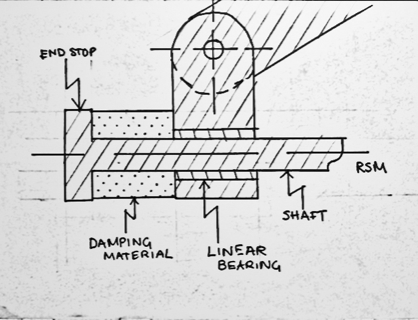
\includegraphics[width=0.5\textwidth]{Images/concepts/ViscoElastic}
    \caption{D1---Viscoelastic damping mechanism.}
    \label{fig:viscoelastic}
\end{figure}

Magnets can also be used to damp vibrations when constrained to a single 
direction. As a permanent magnet travels through a coil, an EMF is induced due 
to Faraday's law, which drives a current when the circuit is complete. The 
current flowing generates a magnetic field opposing the permanent magnet, 
according to Lenz's law. A possible assembly for this system is detailed in 
Figure~\vref{fig:magnetic}. The strength of magnets were to be tuned to the 
desired dynamic properties of the system.

\begin{figure}[H] 
    \centering
    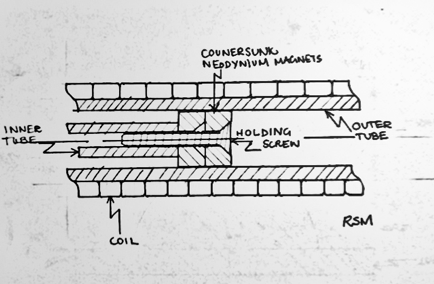
\includegraphics[width=0.5\textwidth]{Images/concepts/Magnetic}
    \caption{D2---Magnetic damping mechanism.}
    \label{fig:magnetic}
\end{figure}

Finally, a simple fluid damping system was considered, whereupon a bearing 
travels through some viscous fluid. Skin friction provides the damping force in 
Figure~\vref{fig:fluidic}. The size of the bearing could be tuned to meet the 
required constraints for damping factor and natural frequency. However, this 
concept was difficult to realise in any manufacturable assembly whilst 
successfully containing the fluid.

\begin{figure}[h] 
    \centering
    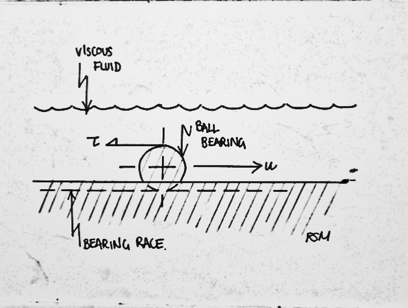
\includegraphics[width=0.5\textwidth]{Images/concepts/Fluidic}
    \caption{D3---Fluidic damping mechanism.}
    \label{fig:fluidic}
\end{figure}

\subsection{Isolation Mechanisms}

Early concepts made use of linkages to transform vertical and lateral 
oscillations into lateral oscillations along damped linear bearings, which 
would have been most easily realised using a viscoelastic damper. 
Figure~\vref{fig:concept1} details one such embodiment.

\begin{figure}[h] 
    \centering
    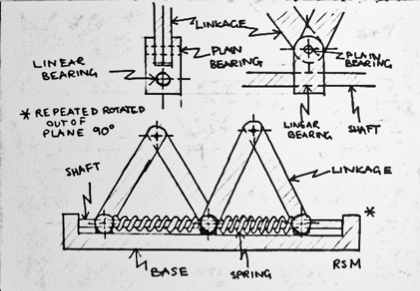
\includegraphics[width=0.5\textwidth]{Images/concepts/Eloise}
    \caption{C1---Simple linkage mechanism.}
    \label{fig:concept1}
\end{figure}

Some components of vertical vibrations were not damped by the mechanism in 
Figure~\ref{fig:concept1}; these were transmitted to the base of the mount such 
that the mount was not completely isolated. Repeating the mechanism by using 
multiple layers of linkages was explored in the concept detailed in 
Figure~\vref{fig:concept2}. Each layer damps a fraction of the vertical 
oscillations transmitted downwards by the layer above resulting in more 
isolation.

\begin{figure}[h]
    \centering
    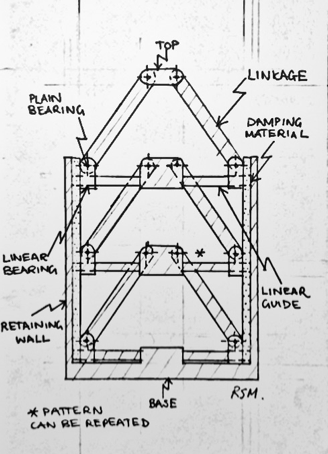
\includegraphics[width=0.4\textwidth]{Images/concepts/RussellLinkage}
    \caption{C2---Layered linkage mechanism.}
    \label{fig:concept2}
\end{figure}

However, the fundamental issue with linkage based isolaton mechanisms is the 
feature size of those linkages. Thin members are prone to resonance with large 
amplitudes at relatively lower frequencies \cite{citation needed}, possibly 
within the audible spectra (20 Hz--20 kHz).

Spherical bearings also featured in design concepts. Figure~\vref{fig:concept3}
describes one such embodiment where a layer of spherical bearings were
sandwiched between two platforms. The upper platform was to be made of a hard 
material such as stainless steel or tungsten carbide, in order to efficiently 
transmit vibrations through to the bearings via point contacts. The bearings 
allowed the top platform to move with the equipment in three degrees of 
freedom: two lateral directions and lateral rotation. The bottom platform would 
have been made of some viscoelastic material with holes for the bearings to 
rest in. Both vertical and lateral oscillations would have been damped by this 
platform and dissipated as heat.

This concept had a major drawback: the damping mechanism was not confined to a 
single degree of freedom. It would have been challenging to determine a single 
damping factor and resonant frequency. The isolation mechanism was an anomaly 
in the concept generation phase, as the damping mechanism was not 
interchangable with those in Section~\vref{sec:damping_mechanisms}.

\begin{figure}[h]
    \centering
    \subfloat[Cross-section]{{
        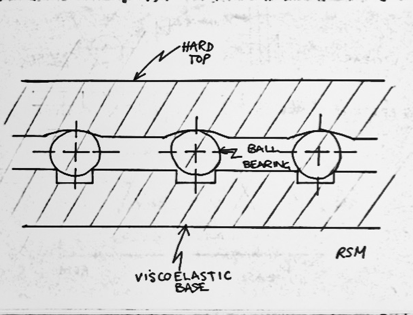
\includegraphics[width=0.4\textwidth]{Images/concepts/George1}
        }}
    \qquad
    \subfloat[Top view]{{       
        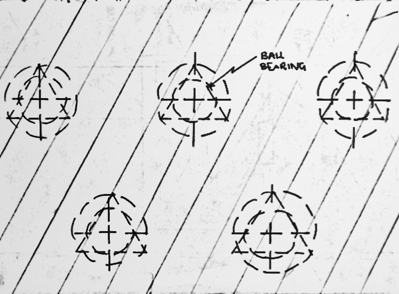
\includegraphics[width=0.4\textwidth]{Images/concepts/George2}
        }}
    \caption{C3---Viscoelastic platform concept.}
    \label{fig:concept3}
\end{figure}

Isolation cones are a popular type of mount, an example is Nordost's Sort 
Kones\textregistered. The Sort Kones are made of three parts: a post, spherical 
bearing, and cone. The bearing rests on the top of the post and the cone sits 
on top of the bearing, such that the cone is free to swivel and rotate. 
However, cones seek only to isolate the mounted equipment and allow free 
movement---they do not attenuate vibrations.

Figure~\vref{fig:concept4} demonstrates how an attenuating mechanism could have 
been incorporated into the post of an isolation cone. The spring in the 
isolation mechanism could have been replaced with one of the damping mechanisms 
in Figure~\ref{fig:viscoelastic} and Figure~\ref{fig:magnetic}.

\begin{figure}[h]
    \centering
    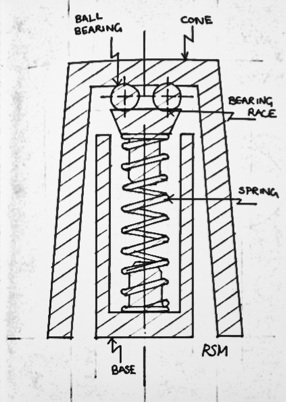
\includegraphics[width=0.4\textwidth]{Images/concepts/Mat}
    \caption{C4---Damped cone concept.}
    \label{fig:concept4}
\end{figure}

An alternative mechanism was devised to translate horizontal and lateral 
oscillations into oscillations of a spherical bearing along a race. 
Figure~\vref{fig:concept5} details the geometry required to achieve this 
translation.

\begin{figure}[h]
    \centering
    \subfloat[Cross-section---maximum load]{{
        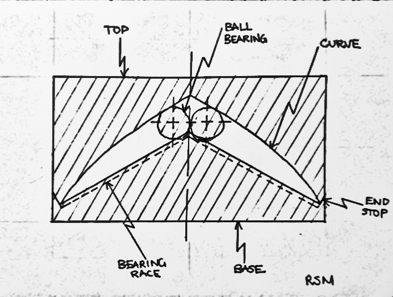
\includegraphics[width=0.4\textwidth,height=0.3\textwidth]{Images/concepts/PointyBottom1}
         }}
    \qquad
    \subfloat[Cross-section---no load]{{
        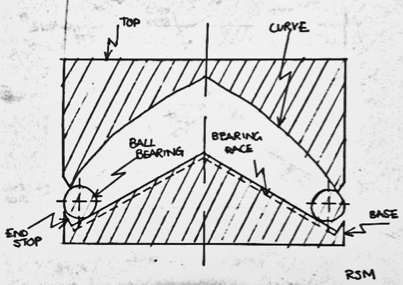
\includegraphics[width=0.4\textwidth,height=0.3\textwidth]{Images/concepts/PointyBottom2}
        }}
    \qquad
    \subfloat[Isometric]{{
        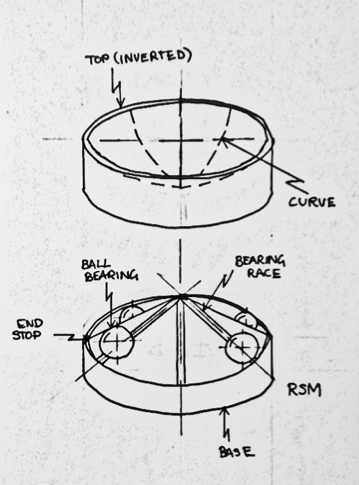
\includegraphics[width=0.35\textwidth]{Images/concepts/PointyBottom3}
        }}
    \caption{C5---Cone and bearing concept.}
    \label{fig:concept5}
\end{figure}


When no force is applied to the top piece, the bearing would travel to the 
bottom of its race. Increasing the load would cause the bearing to move up the 
race due to the gradient of the curve on the top piece, which was greater than 
the gradient of the race. There would be some component of the reaction force 
acting on the bearing perpendicular to the curve which points up the the slope 
of the race. However, the gradient of the curve decreases travelling up the 
slope, so for a given load the component of the reaction force would also 
decrease. Therefore, for each load, there is a different equilibrium position 
somewhere along that race where the components of the bearing's weight and the 
reaction force acting on the bearing in the direction of the race are equal and 
opposite. The mechanism acts as a geometric spring with some stiffness.

The frictional sheer forces in the mechanism would provide significant damping 
due to the magnitude of the reaction forces involved. Furthermore, one of the 
damping mechanisms in Figure~\ref{fig:viscoelastic} or 
Figure~\ref{fig:magnetic} could be coupled to the linear motion of the 
bearings to tune the system to a desired natural frequency and damping 
factor---this could result in quite a large footer.

A drawback of this concept is difficulty in containing the bearings, the user 
would be free to remove the top piece, and the bearings would all come out of 
their races. Competitors could easily see how the mechanism works and replicate 
it for themselves.

Figure~\vref{fig:concept6} details a variation of C5, whereby the bearings 
travel outwards up the slope. This creates more space for a damping mechanism 
for each race around the outside of the footer. A fluid could be contained in 
the cavity in the bottom piece to damp vibrations using the mechanism described 
in Figure~\ref{fig:fluidic}.

\begin{figure}[h]
    \centering
    \subfloat[Cross-section---maximum load]{{ 
        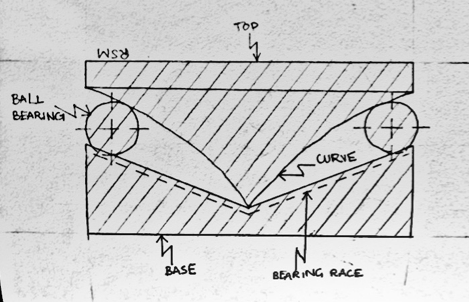
\includegraphics[width=0.4\textwidth,height=0.3\textwidth]{Images/concepts/PointyTop1}
        }}
    \qquad
    \subfloat[Cross-section---no load]{{
        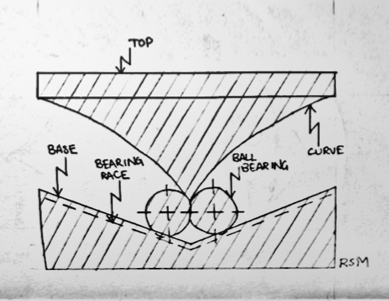
\includegraphics[width=0.4\textwidth,height=0.3\textwidth]{Images/concepts/PointyTop2}
        }}
    \qquad
    \subfloat[Isometric]{{
        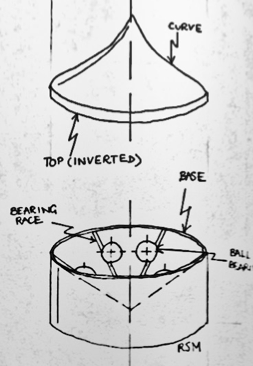
\includegraphics[width=0.3\textwidth]{Images/concepts/PointyTop3}
        }}
    \caption{C6---Alternative cone and bearing concept.}
    \label{fig:concept6}
\end{figure}

The flexibility of the alternative cone and bearing concept C6, coupled with 
its innovative design set the concept apart from its alternatives. In 
\cite{maguire2016vibration}, it was shown how concept C6 with damping mechanism 
D2 best matched the customer's expectations and engineering requirements. This 
is the concept which informed the next stage of development and our final 
design.

\section{Design Development}

Through an iterative process, the concept highlighted in 
\cite{maguire2016vibration} for its promise was increasingly refined to produce 
a final design. The key milestones in development are as follows:

\begin{itemize}
    \item The transition from curved geometry to opposing pairs of rare earth 
    magnets to support the equipment's weight.
    \item The addition of a user-adjustable preloading mechanism to increase 
    the range of masses that could be supported to full mass range of 
    amplifiers: 5~\si{\kilogram}--30~\si{\kilogram}~\cite{citation needed}.
    \item The casing required to contain the isolation mechanism and dissuade 
    the user from dismantling the footers.
    \item The choice of materials used for various parts in the system.
    \item The development of the models used to tune the design to meet 
    performance requirements.
\end{itemize}

\subsection{Opposing Magnets}

Early in the development process, it became apparent the curved geometry of 
concept C6 in Figure~\ref{fig:concept6} would not be able to support a 
particularly wide range of masses. Initially, a ring magnet mounted on the end 
of a rod was to be coupled to the bearings to damp oscillations, biased using a 
compression spring---see Figure~\ref{fig:magnetic}.

To simplify the design and increase the supported mass range, the inclined 
bearing races in the base and curve in top piece were removed, and replaced 
with flat bearing races and a cone respectively. The damping mechanism was 
replaced with six pairs of opposing rare earth button magnets, with the 
opposing poles of magnets in adjacent races changing from N--N to S--S to N--N 
etc. The direction of poles alternate to allow the flux to flow in closed 
loops, and avoid flux leakage out of the system. Hysteresis losses in the base 
piece and frictional forces provide the damping forces in this system.

Figure~\vref{fig:rev1} shows how the magnets and bearings would be arranged in 
a mount with opposing magnet pairs. These drawings have six races for a 
multitude of reasons:
\begin{itemize}
    \item The number of opposing pairs had to be an even number to allow the 
    poles of magnets in adjacent races to point in alternating directions for 
    \emph{all} races. Otherwise the behaviour of the repulsive forces in some 
    races would be different the others.
    \item At least four races were required to allow freedom of movement in 
    both lateral directions.
    \item Using more races would require a larger diameter for the same usable 
    travel distance.
    \item Finally, because the magnetic repulsion force is not a linear 
    function of separation distance, oscillations parallel with a race would 
    experience a greater stiffness than those between races. Mounts with more 
    races would have less variation in lateral stiffness in different lateral
    directions.
\end{itemize}

\begin{figure}[h]
    \centering
    \textbf{ISOMETRIC OF INITIAL CAD REVISION}
    \textbf{CROSS-SECTION OF INITIAL CAD REVISION}
    \caption{Isometric view and cross-section of inital design revision.}
    \label{fig:rev1}
\end{figure}

The choice of six races was a compromise between the size of the mount and 
having a mount with a more constant stiffness in different lateral directions.

\subsubsection{Flux Path Simulation}

As the footer houses twelve rare earth magnets, considerations have to be made 
for the way in which these magnets interact with the surroundings of the footer 
as they could cause damage or interfere with mounted or surrounding 
equipment footer. Using a software package called 
MagNet\textsuperscript{\textregistered} produced by 
infolytica\textsuperscript{\textregistered}, it was possible to perform a 2D 
finite element analysis of the footers, allowing the effects of these magnets 
to be modelled. The analysis performed in this section is for the geometry of 
the final design, but the same procedure was performed following each 
significant revision during the design process. When modelling the effect of 
these magnets the two extreme cases were considered: at minimum and maximum 
separation as detailed in Figure~\ref{figure:minsep} and 
Figure~\ref{figure:maxsep}.

\begin{figure}[h]
    \centering
    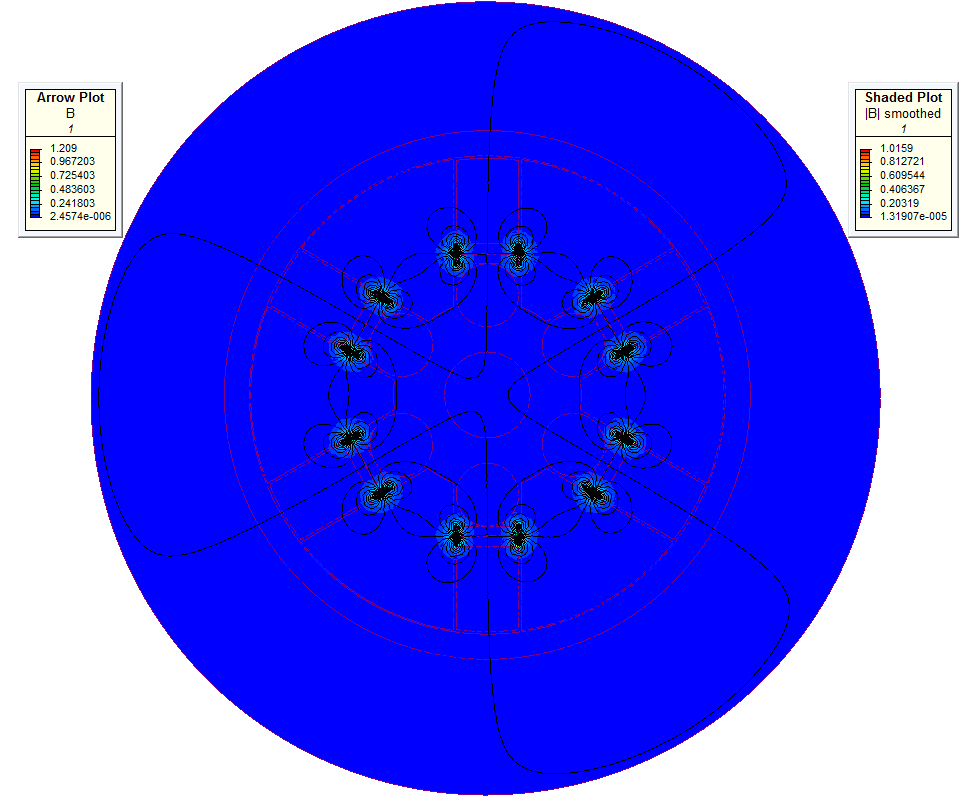
\includegraphics[width=\textwidth]{Images/maxpreload.png}
    \caption{Flux state with minimum separation of magnets}
    \label{figure:minsep}
\end{figure}

\begin{figure}[h]
    \centering
    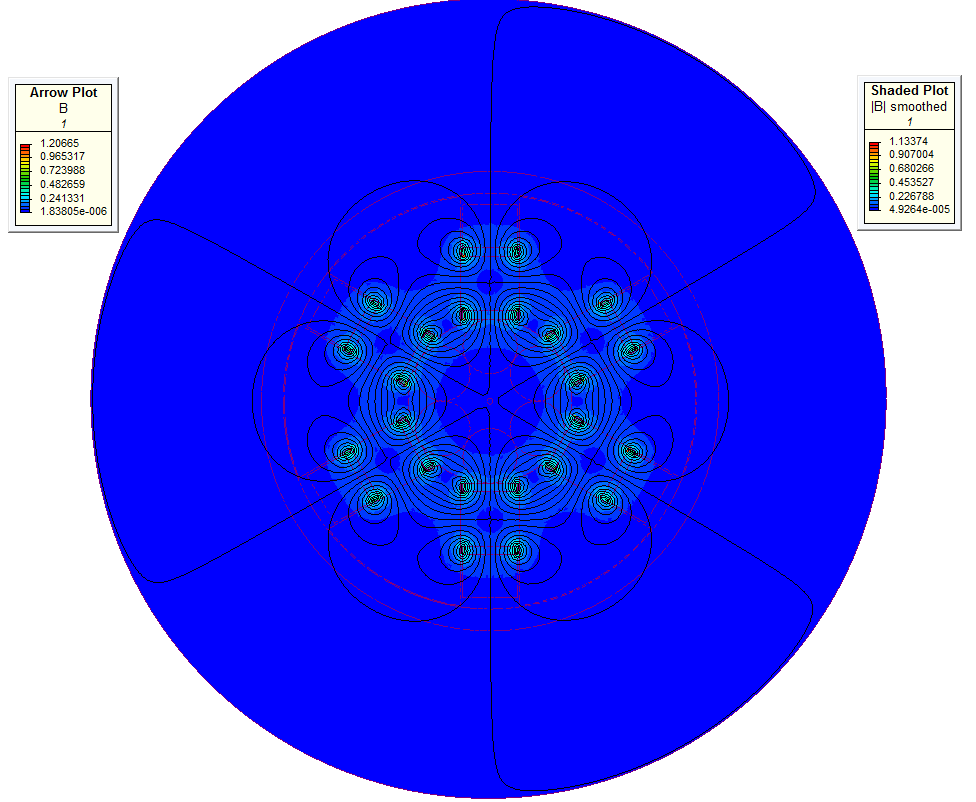
\includegraphics[width=\textwidth]{Images/minpreload.png}
    \caption{Flux state with maximum separation of magnets}
    \label{figure:maxsep}
\end{figure}

It can be seen that the flux density outside of the footer is negligible as it 
has a value of the order $10^{-5}$~\si{\tesla} meaning that there would be 
minimal to no interactions between the footer and its surroundings as nearly 
all of the magnetic flux is contained within the core of the device.

\subsubsection{Magnetic stresses}

The opposing pole pairs of magnets housed within the core of the design exist 
in a highly stressed state, meaning that the force applied to each magnet is 
large and has to be considered. The maximum force acting between the magnets is 
$p_{m\,max}$ and from this the maximum stress within the magnet could be 
calculated. This was shown to be 0.175~\si{\mega\pascal} and the yield stress 
3.96~\si{\mega\pascal} meaning that there is a factor of safety of 23 per 
magnet. This suggeststhese magnets will not structurally fail during the 
operation of this product.

\subsection{Preloading Mechanisms}
\subsection{Casing}

\subsection{Materials}

Neodymium magnets are the most widely used type of rare-earth magnet, strongest 
type of permanent magnet commercially available and of greatest benefit in 
applications where there is limited space---such as for the opposing magnet 
pairs in these footers.

Tungsten carbide possesses a Young's modulus of 530~\si{\giga\pascal}, more 
than two times of that of AISI 316 stainless steel; a material commonly used 
for spherical bearings. Due to Hooke's law, the material does not undergo large 
deflections which in turn ensures efficient energy transfer between the Hi-Fi 
components. The bearings do not require any lubrication as they grind down any 
particulates that may enter the system. Tungsten carbide was selected for the 
bearings in this project.

With regards to the custom machined parts, there are two options: AISI 304 
stainless steel and 6061-T6 \emph{aircraft-grade} aluminium. Stainless steel is 
harder so, in a similar way to tungsten carbide, is a more efficient 
transmitter of vibrations. It is also harder wearing so more suitable for 
moving parts. Aluminium, being softer, is cheaper to cut. A part machined in 
stainless steel will cost around 30\% more than the same part machined in 
aluminium~\cite{citation needed}, given there are no delicately thin features 
which would benefit from the stronger material.

Considering this, the aluminium alloy was selected for the purely structural 
parts, leaving 304 stainless steel for the core part (COR080-0003) which the 
bearings are contained in and flux must be able to travel through; the top 
piece (TOP080-0004) which pushes the bearings along the race; and the user 
replaceable spike (USR080-0001) which the vibrations are conducted through.

\subsection{Screw Specification}

The design features seven screws, six of which are to be used to attach the 
retaining wall to the core, with the other being used as a means of preloading 
the system. All of these screws are to be made of A2 tool steel which has a 
yield stress, $\sigma_{y}$, of 205~\si{\mega\pascal} in compression and 
therefore through the Von Mises yield criterion it is possible to achieve its 
yield stress in shear. The yield criterion is as follows:
\begin{equation}
    k = \frac{\sigma_{y}}{\sqrt{3}}
\end{equation}
where $k$ is the stress at failure. For A2 tool steel this value 
is 118~\si{\mega\pascal}.

Due to the nature of the retaining wall used to constrain the preloading 
backstops in their tracks, there is a shear force applied to the six retaining 
wall screws. At the worst possible instance the shearing force on one of these 
screws was a sixth of the total weight resting on the footer. It was decided 
that a single footer should not structurally fail in the event of a person 
accidentally stepping on it, meaning that these six retaining wall screws were 
specified to withstand the weight of a 140~\si{\kilogram} mass between them.

Reference~\cite{blake1986every} recommends preloading the screw to twice 
of the applied load in order to increase the friction between the core and 
the screw and increase the screw's resistance to loosening. Hence, the total 
load applied to the screw is the sum of the preload and the applied 
load---this equates to 700~\si{\newton}.

The stress analysis was performed on the screws to find what diameter would be 
required such that the screws could meet this specification. The screws' 
interaction with the core piece allowed for them to be modelled as a cantilever 
with a uniformly distributed load across its top edge as can be seen in 
Figure~\vref{fig:screw}. Using this model the maximum shear stress within 
the screw was considered for various diameters of ISO  metric threads, the 
results of the analysis can be seen in Table~\vref{table:stresses-retainer}.

\begin{figure}[h]
    \centering
    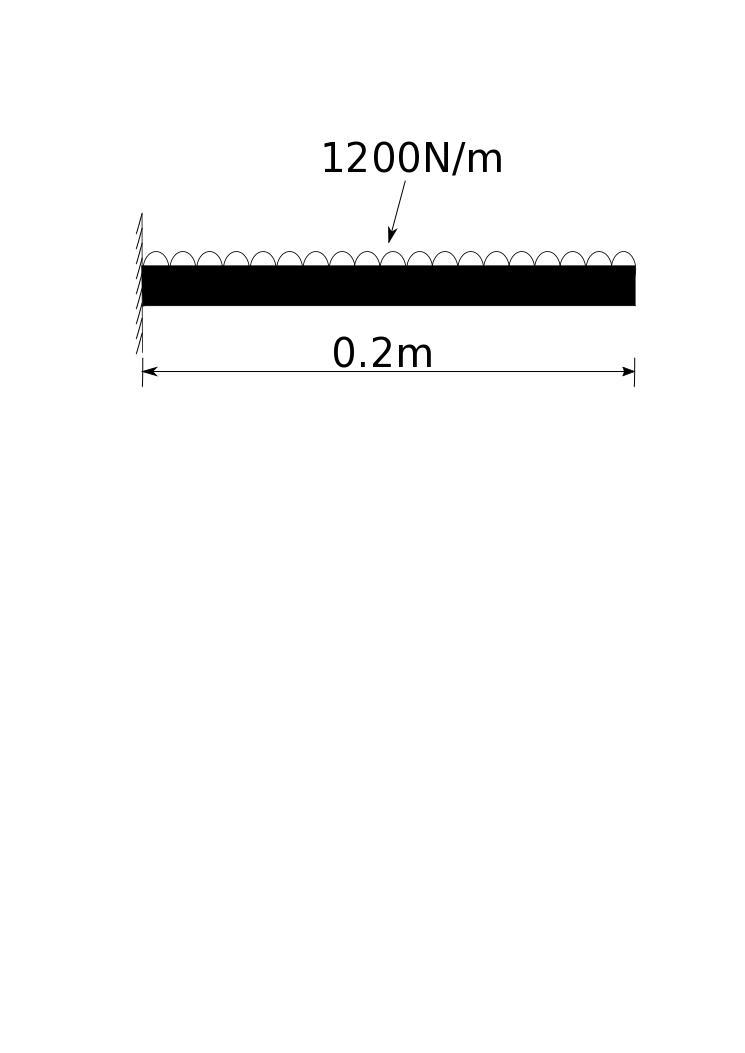
\includegraphics[width=0.5\textwidth]{Images/retainerscrew.png}
    \caption{Load applied to retaining wall screws.}
    \label{fig:screw}
\end{figure}

\begin{table}[h]
    \centering
    \caption{Stress concentration analysis of the retainer screws.}
    \begin{tabular}{cccc}
        \toprule
        Thread & D\,/\,\si{\milli\meter} & $\tau$\,/\,\si{\mega\pascal} & 
        Suitable\\
        \midrule
        M1.6 & 1.25 & 586.8 & No\\
        M2 & 1.60 & 358.1 & No\\
        M2.5 & 2.05 & 218.1 & No\\
        M3 & 2.50 & 146.7 & No\\
        M3.5 & 2.90 & 109.0 & Yes\\
        M4 & 3.30 & 84.2 & Yes\\
        \bottomrule
    \end{tabular}
    \label{table:stresses-retainer}
\end{table}

When considering the preloading screw at the bottom of the footer, the load was
applied along its top edge, so it was modelled as a strut with a single 
point load on top. Again, the worst possible case of applied load to the screw 
was the full 140~\si{\kilogram} mass being supported by it as may be seen in 
Figure~\vref{fig:preload-screw}. Therefore, the maximum stress case within the 
screw was considered for this applied load and tested for various diameters 
of ISO metric threads, as can be seen in Table~\ref{table:stresses-prelaod}.

\begin{figure}[h]
    \centering
    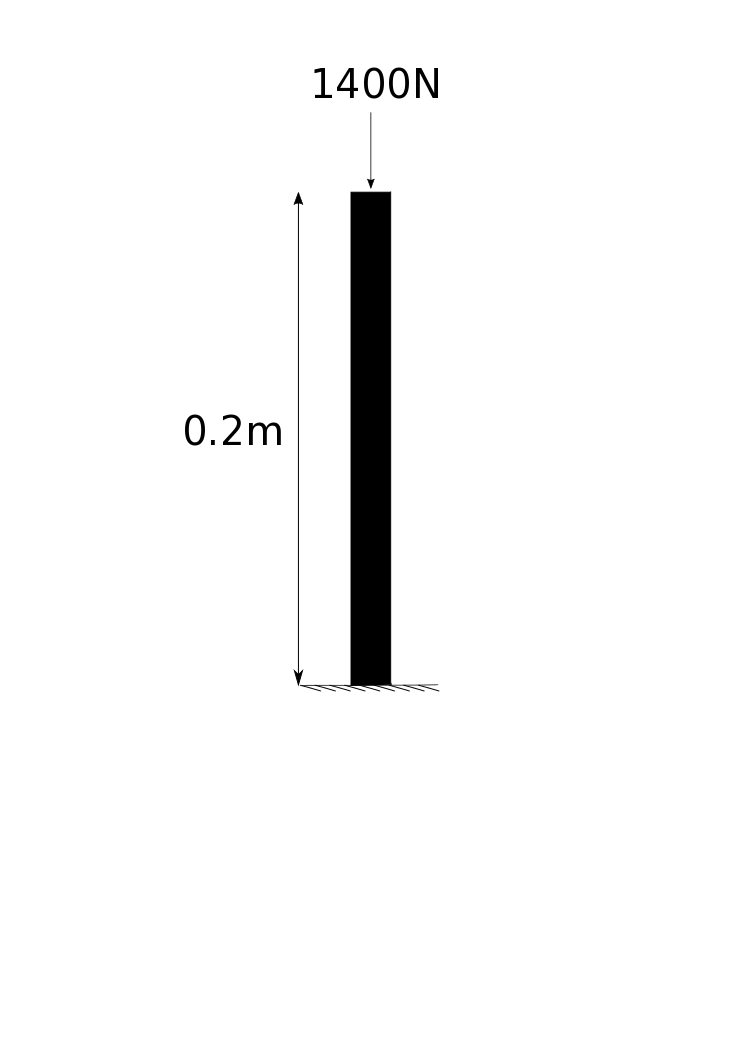
\includegraphics[width=0.5\textwidth]{Images/preloadscrew.png}
    \caption{Load applied to the preload screw.}
    \label{fig:preload-screw}
\end{figure}
	
\begin{table}[h]
    \centering
    \caption{Stress concentration analysis of the preload screw}
    \begin{tabular}{cccc}
        \toprule
        Thread & D\,/\,\si{\milli\meter} & $\tau$\,/\,\si{\mega\pascal} & 
        Suitable\\
        \midrule
        M1.6 & 1.25 & 1140.0 & No\\
        M2 & 1.60 & 696.3 & No\\
        M2.5 & 2.05 & 424.4 & No\\
        M3 & 2.50 & 285.2 & No\\
        M3.5 & 2.90 & 212.0 & No\\
        M4 & 3.30 & 163.7 & Yes\\
        M5 & 4.20 & 101.1 & Yes\\ 
        M6 & 5.00 & 71.3 & Yes\\
        \bottomrule
    \end{tabular}
    \label{table:stresses-preload}
\end{table}

As can be seen from Table~\ref{table:stresses-retainer} and 
Table~\ref{table:stresses-preload}, for both cases an M4 thread screw meets the 
specification and therefore shall be used in the design. By specifying the 
screws for a 140kg mass per piece, there has been a large factor of safety 
considered for the pieces as the maximum mass which the design has been 
specified to work for is a 44.6kg mass supported by three footers meaning that 
the screws have a factor of safety of at least 9.4.

The final design contained a preloading mechanism which relied upon the user 
being able to operate the preloading screw. To ensure that the torque required 
to operate this screw was within human capabilities a static analysis was 
performed. The factors which effect the torque required to preload the system 
are: the coefficient of friction $\mu$ between the screw and its mating 
thread; the nominal bold diameter $D$ and the bolt tension $P$. The required 
torque $T$ is given by the following:
\begin{equation}
    T = \mu D P
    \label{eq:screw-torque}
\end{equation}  
    For stainless steel, $\mu$ is 0.8 and for the M4 screw, $D$ is 
4~\si{\milli\meter}. From Figure~\ref{fig:nomenclature} it can be seen that 
there is a force $p_m$ applied horizontally through the preloading backstop 
that causes a resultant force $P/6$ acting on each of the six vertical struts 
of the crown. These forces were resolved find $P/6$:
\begin{equation}
    \frac{P}{6} = p_m tan(\beta)
    \label{eq:resolve-preload}
\end{equation}
where $\beta$ was 60.04\si{\degree}.

To preload the system, the user has to remove all load from the footer, so the 
bearings will rest at a maximum distance away from the backstop. The magnetic 
repulsion force $p_m$ reaches a maximum when the magnet separation is at a 
minimum---at maximum preload. This value $p_{m\,max}$ was 1.23~\si{\newton}. 
Equation~\ref{eq:resolve-preload} was substituted into 
Equation~\ref{eq:screw-torque}:
\begin{equation}
    T_{max} = 6\,\mu\,D\,p_{m\,max}\,tan(\beta)
    \label{equation:screw-torque2}
\end{equation}
which yielded a $T_{max}$ value of 0.053~\si{\newton\meter}, well within human 
capabilities given \cite{stokes1976man} quotes the 5th percentile for 
maximum torque strength as 7.21~\si{\newton\meter}.

\subsection{Dynamic Analysis}
\subsubsection{Parametric Model} \label{sec:parametric-model}
\subsubsection{System Tuning}
\subsubsection{Experimentation} \label{sec:experimentation}

To assess the effectiveness of the product, acceleration data from a vibrating 
amplifier was recorded to determine the frequency content of the signal to be 
attenuated. The same setup was used to capture acceleration data from the 
amplifier when mounted on half squash balls, which was later compared to the 
output of a dynamic model representing the final mount design using the 
undamped acceleration data captured as the model input. Squash balls were used 
to isolate Hi-Fi systems before footers entered the market and are an entry 
level alternative to footers.

A USB PicoScope\footnote{Pico Technology PicoScope 2204A} was used to capture 
the output of an accelerometer\footnote{STMicroelectronics LIS344ALH} at a 
sample rate of 50~\si{\kilo\hertz} for 10~\si{\second}. Human hearing ranges 
from 20~\si{\hertz}--20~\si{\kilo\hertz}; according to Nyquist, the sample rate 
had to be at least twice 20~\si{\kilo\hertz} to determine the power of these 
frequency components. 

The accelerometer was coupled to the top of an amplifier connected to a 
standard AC mains power supply---nominal voltage of 240~\si{\volt} at a 
frequency of 50~\si{\hertz}. Data from the accelerometer was captured for three 
conditions: with the amplifier turned off, on, and the amplifier turned on 
whilst sitting on half squash balls.

The data captured came in the form of a voltage output. To determine the 
acceleration from this information it was necessary to form a transfer
equation. To do so, the technical data sheet for the accelerometer 
\cite{SensorManual} was found and in it there was clear conversion which lead 
to the following
\begin{equation} \label{eq:acceleration}
    \ddot{y} = 9.81\cdot(0.66\cdot V - 1.65)
\end{equation}
where $a$ is the acceleration in \si{\meter\per\square\second} and $V$ is the 
voltage measured in \si{\volt}. Equation~\ref{eq:acceleration} is linear, so 
has no affect on the shape of the spectra. The spectra of the measured voltages 
were analysed instead.

Firstly, the data for the amplifier when off---the control---was compared to 
the amplifier when on; their spectra up to 1~\si{\kilo\hertz} are shown in 
Figure~\vref{fig:MatGraphs1}. There were no observable components above the 
noise floor in the range 1~\si{\kilo\hertz}--25~\si{\kilo\hertz}.

\begin{figure}[h]
    \centering
    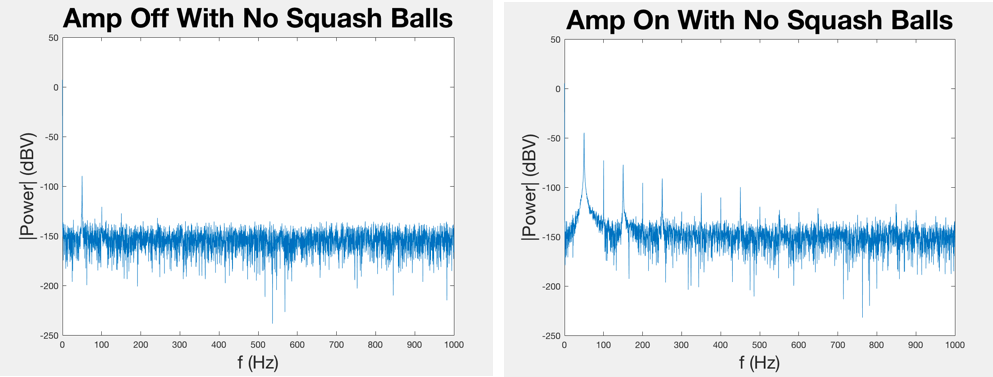
\includegraphics[width=\textwidth]{Images/MatGraphs}
    \caption{Compared Frequency Responses when Amplifier off and on}
    \label{fig:MatGraphs1}
\end{figure}

The spectra for amplifier when off had a fundamental at 50~\si{\hertz}. This is 
likely due to interference from other mains powered devices in the room---air 
conditioning, PCs and desktop power supplies for example. Contrasting this 
control spectra to the spectra for the amplifier when turned on, the 
fundamental frequency increased in power significantly from $-90$~\si{dBV} to 
$-40$~\si{dBV}---a factor of $10^5$. The harmonics can be seen at 
50~\si{\hertz} intervals although the noise floor due to the error of the 
accelerometer remained at $-140$~\si{dBV}.

Next, the spectra for the amplifier when on was compared to the spectra for the 
amplifier damped using squash balls. Figure~\vref{fig:MatGraphs2} reveals the 
effect the squash balls had on the frequency content of observed vibrations. 

The fundamental remains constant in frequency and power. However, from the 
simple damping the squash balls provide, the noise has been significantly 
cleared up, along with this success the harmonics have consistently lower 
peaks. This provides an example of successful damping which can be used as a 
comparison to the later mathematically damped data using dynamic model. The aim 
is to further clean up the noise and lower the power of the harmonics as much 
as possible, preferably below the noise floor which should lead to a reduction 
in microphonic effects and increase in sound quality.

\begin{figure}[h]
    \centering
    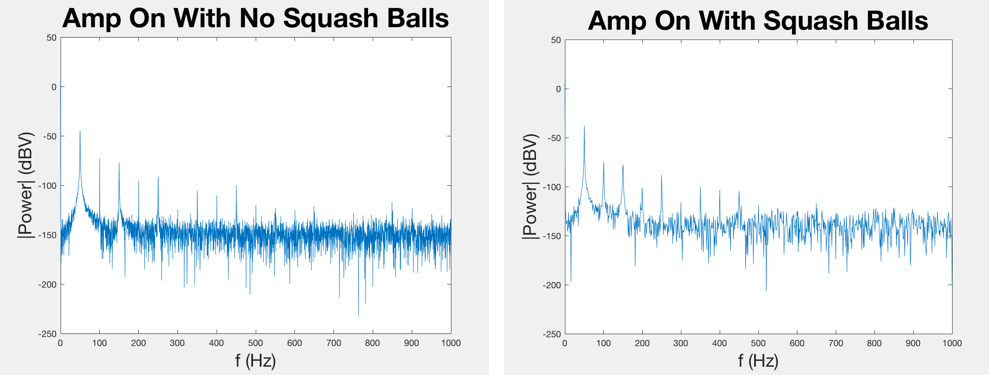
\includegraphics[width=\textwidth]{Images/MatGraphs2}
    \caption{Compared Frequency Responses with and without Squash Balls}
    \label{fig:MatGraphs2}
\end{figure}

\subsubsection{Dynamic Simulation}

It was determined that a dynamic model of the system would be necessary to 
quantify the potential success of the product. This could visually display the 
effects of the footers on attenuation of a signal from a Hi-Fi system, and 
hence inform whether the sound quality would be improved.

The three footers and mounted equipment can be simplified to a spring-mass 
damper system with non-linear stiffness---a driving force $F_d$ is supplied by 
the vibration of the Hi-Fi system, and the opposing forces from the magnetic 
repulsion force $F_m(y)$, damping force $c\dot{y}$ and system inertia 
$m\ddot{y}$. Considering these components, it was possible to develop a second 
order differential equation which when solved would characterise the 
effectiveness of the footers.
\begin{equation} \label{eq:2ndDiff}
    F_d = m\ddot{y} + c\dot{y} + F_m(y) 
\end{equation}

Simulink\textsuperscript{\textregistered} was chosen to drive the dynamic model 
due to the straight-forward construction of differential equations it provides; 
it offers a visual representation of the system and works hand-in-hand with 
MATLAB allowing for simple data processing. Simulink computes an iterative 
numerical solution and outputs a corresponding time series to the MATLAB 
workspace which can be transformed into the frequency domain for analysis.

Four components needed to be defined to complete the model:
\begin{itemize}
    \item The mass of the supported equipment and top piece $m$. The simulation 
    was run on the nominal supported mass of 20~\si{\kilogram}.
    \item Constant $c$, which is dependent on the supported mass and the 
    frictional coefficient $\mu$ between the tungsten carbide balls, and 
    stainless steel cones and races for all three footers.
    \item A transfer function $F_m(y)$ to find the magnetic repulsion force 
    given the vertical displacement of the equipment.
    \item $F_d$ which varies with time and the input to the system, found by 
    applying Newton's second law to the undamped accelerations measured in 
    Section~\ref{sec:experimentation}.
\end{itemize}

Section~\ref{sec:parametric-model} details how the magnetic repulsion force can 
be calculated given the vertical displacement of the equipment using
Equation~\ref{eq:?}. This was implemented as a subsystem in Simulink, 
incorporating transformations necessary to determine magnet separation given 
horizontal displacement; repulsion force acting on a single bearing given 
magnet separation; and total reaction force given the force acting on a single 
bearing.

Ideally the damping coefficent for various masses would be determined 
empirically, however, using the theoretical approach outlined in 
Section~\ref{sec:parametric-model} the damping coefficient was found for a range
friction coefficients $\mu$. Typically for these materials $0.4 < \mu < 0.6$. 
Substituting the limits and nominal mass into Equation~\ref{?}, the damping 
coefficient was bounded as follows
\begin{equation*}
    159~\si{\newton\second\per\meter} < c < 238~\si{\newton\second\per\meter}
\end{equation*}

Figure~\vref{fig:MatModel} displays the top level model architecture. The 
topology is typical of spring mass damper systems as detailed in 
\cite{mass2017matlab}.

\begin{figure}[h]
    \centering
    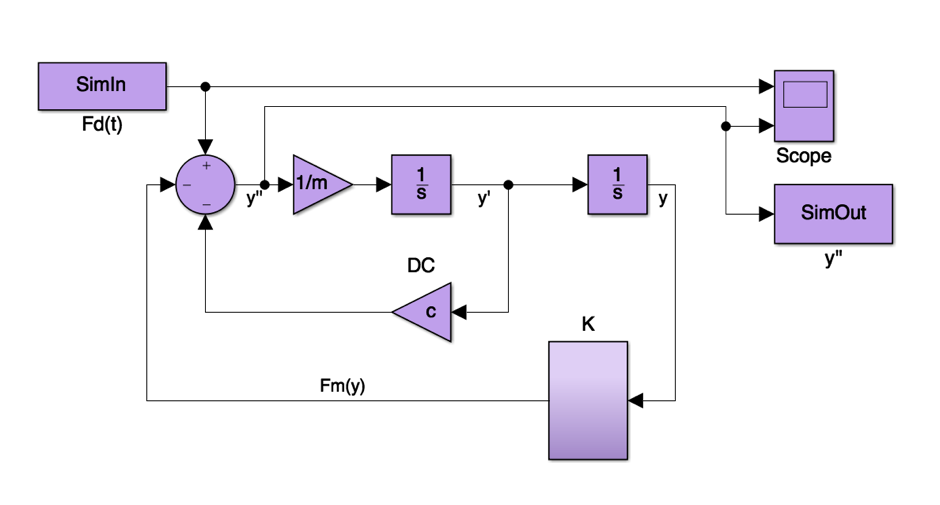
\includegraphics[width=0.8\textwidth]{Images/MatModel}
    \caption{Compared Frequency Responses with and without Squash Balls}
    \label{fig:MatModel}
\end{figure}

The constant stiffness was replaced with the subsystem used to find the 
magnetic repulsive force. \emph{SimIn} provided an interface to the MATLAB 
workspace which was used to input the driving force. Similarly, \emph{SimOut} 
exported the system output to the workspace; the acceleration of the equipment 
as a time series. Using the inverse of Equation~\vref{eq:acceleration}, the 
model output was converted into voltages so its spectra could be compared to 
the accelerometer output measured for the undamped amplifier.

Figure~\vref{fig:CoF} shows the effect of running the simulation with the 
damping coefficient at each extreme. 

\begin{figure}[h]
    \centering
    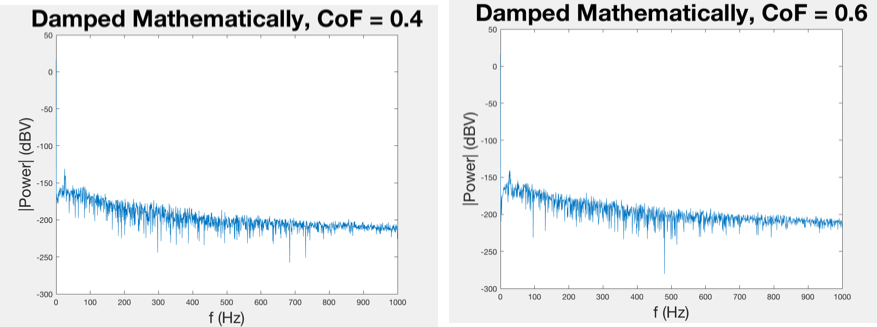
\includegraphics[width=\textwidth]{Images/MatGraph3}
    \caption{Power Output for Coefficient of Friction Extremes}
    \label{fig:CoF}
\end{figure}

In both graphs, the fundamental frequency can no longer be observed; a peak at 
around 30~\si{\hertz} is apparent however its low power and frequency that 
differs from 50~\si{\hertz} indicate that this is just noise. The noise is 
effectively identical in both cases and hence it can be concluded that the 
difference in damping coefficient across its range negligible effect. For 
further analysis, the median coefficient of friction will be used---0.5---this 
returns a damping coefficient of 198~\si{\newton\second\per\meter}.

The undamped is displayed with the simulation output damped spectrum for 
comparison between the input and output of the dynamic model in 
Figure~\ref{fig:DampedVUndamped}.

\begin{figure}[h]
    \centering
    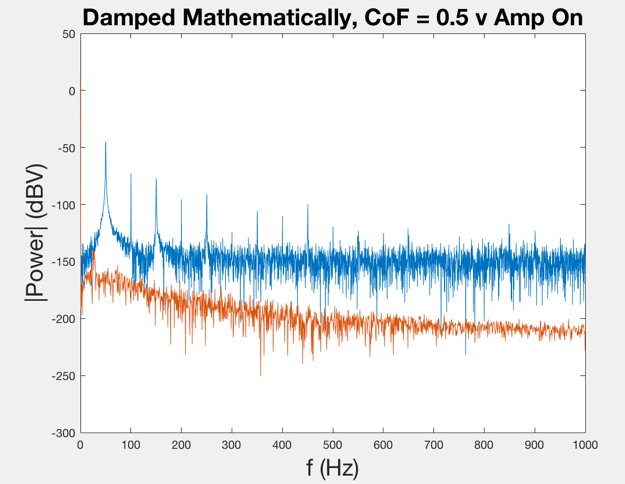
\includegraphics[width=0.8\textwidth]{Images/MatGraph4}
    \caption{Comparison of Undamped and Damped Response}
    \label{fig:DampedVUndamped}
\end{figure}

The red curve shows the simulation output; the fundamental frequency and its 
harmonics are indistinguishable from the noise. The entire signal has been 
reduced to below the noise floor of around $-140$~\si{dBV}. The noise has been 
almost completely attenuated.

The success of the footers is likely to be less significant than that of the 
model. The primary reason for this discrepancy is the value of damping 
coefficient used. Ideally, this would be found empirically; a series of 
prototypes would be produced and a similar experiment carried out to find the 
true damping coefficient.

If the footers have a fraction of the successs they have been predicted to 
have, there will be a significant improvement in sound quality. 

\section{Detail Design} \label{sec:DetailDesign}

\subsection{Mounting}

\subsection{Rails}

\subsection{Finishes}

\section{Design for Manufacture} 

DFM defines the design of a product so as to best optimise its quality whilst minimising its cost to manufacture\cite{dfm}. Factors affecting this cost include the number of off-the-shelf and machinable parts, the set-up time of required machinery, the material type, dimensional tolerances as well as secondary processes. Generally, a compromise is reached between the functional quality of a product and the cost of manufacture however, considering the current extortionate pricing of similar existing products, certain design choices have taken precedence over their implications in a manufacturing context, for the example the rails within the complex central piece are undesirable to manufacture(see drawing COR080-0003) yet optimal for the specified mechanism.

\subsection{Bill of Materials}

Figure~\ref{fig:bom-labels} labels all of the parts used in the final design, 
including the added user replaceable parts: the spike and base. These are 
described in Table~\ref{table:bom}.

\begin{figure}[H]
    \centering
    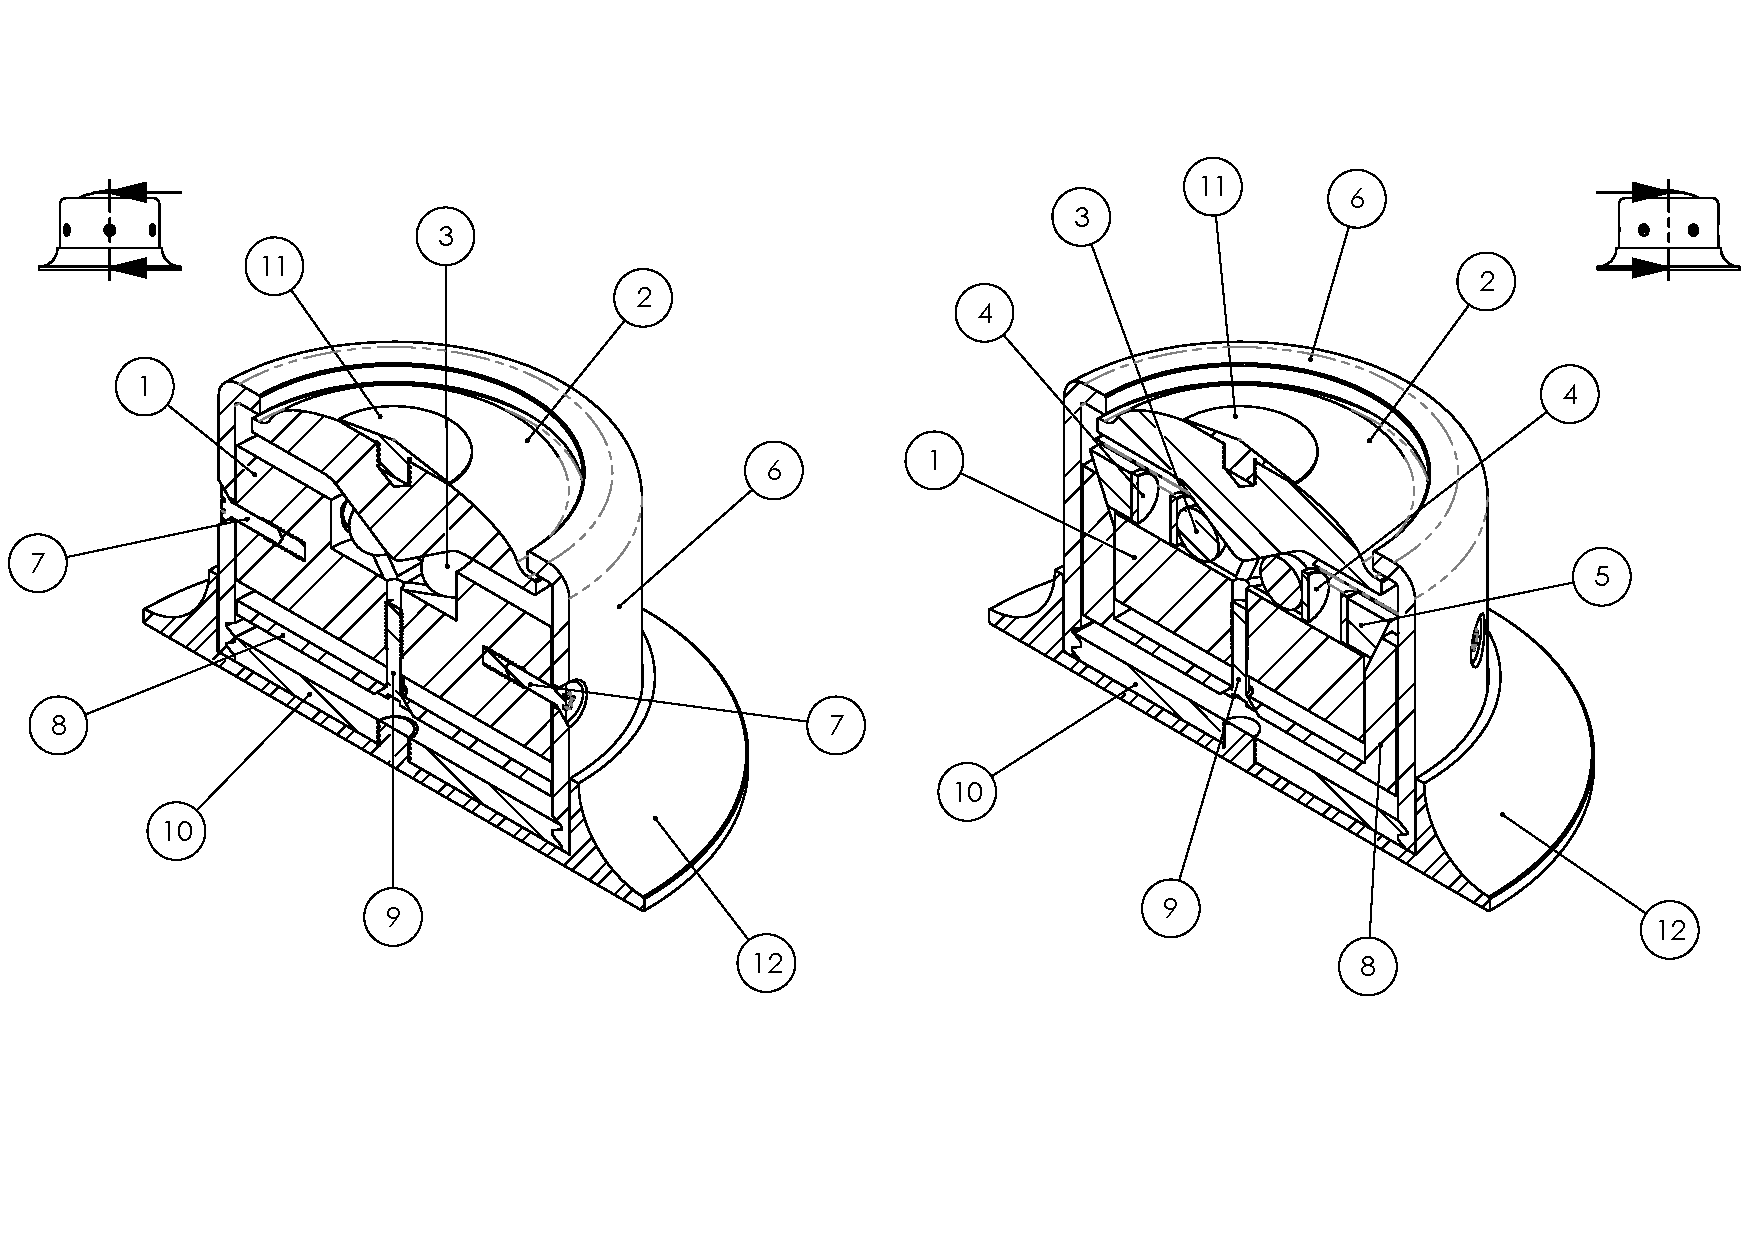
\includegraphics[width=\textwidth]{Images/ISO080-ASM-USR.PDF}
    \caption{Item numbers for Table~\ref{table:bom}.}
    \label{fig:bom-labels}
\end{figure}

\begin{table}[H]
    \centering
    \footnotesize
    \begin{threeparttable}
        \caption{Bill of Materials}
        \label{table:bom}
        \begin{tabular}{@{}clp{17em}c@{}}
            \toprule
            Item No. & Part No. & Description & Qty. \\
            \midrule
            1 & COR080-0003 & \raggedright Isofonics core piece & 1 \\
            2 & TOP080-0004 & \raggedright Isofonics top piece & 1 \\
            3 & 10MMTUNGSTENBALLS\tnote{1} & \raggedright \diameter 10~mm 
            tungsten carbide ball & 6 \\
            4 & F669-N45SH-10\tnote{2} & \raggedright \diameter 10~x~1.5~mm 
            neodymium 
            button magnet & 12 \\
            5 & PLD010-1004 & \raggedright Isofonics preloading back-stop & 1 \\
            6 & RET080-0003 & \raggedright Isofonics retainer & 1 \\
            7 & M4X20-CSK-ST\tnote{3} & \raggedright M4~x~20~mm T20 A2 c'sunk 
            screw with partial thread & 6 \\
            8 & PLD080-0003 & \raggedright Isofonics preloading crown & 1 \\
            9 & M4X20-CSK-H\tnote{4} & \raggedright M4~x~20~mm H2.5 A2 c'sunk 
            screw with partial thread & 1 \\
            10 & RET080-1002 & \raggedright Isofonics retainer bottom & 1 \\
            11 & USR080-0001 & \raggedright Isofonics removable spike & 1 \\
            12 & USR080-1002 & \raggedright Isofonics removable base & 1 \\
            \bottomrule
        \end{tabular}
        \begin{tablenotes}
            \raggedright
            \tiny
            \item[1]\url{http://www.vxb.com/10mm-Tungsten-Carbide-Bearing-Ball-0-3937-inch-Dia-p/10mmtungstenballs.htm}
            \item[2]\url{http://www.first4magnets.com/circular-disc-rod-magnets-c34/10mm-dia-x-1-5mm-thick-n45sh-neodymium-magnet-1-1kg-pull-p3633}
            \item[3]\url{http://www.westfieldfasteners.co.uk/A2_ScrewBolt_PinTXCsk_M4.html}
            \item[4]\url{http://www.westfieldfasteners.co.uk/A2_ScrewBolt_SHCsk_M4.html}
        \end{tablenotes}
    \end{threeparttable}
\end{table}

\subsection{Off-The-Shelf Parts}
Due to the complex geometry required from our design, only few components may be bought in, namely (per mount);  six �10mm tungsten carbide ball bearings, six \diameter 10 x 1.5 mm neodymium magnets, six M4 by 20 mm AISI A2 steel countersunk Torx security screws and one M4 by 20 mm countersunk hex socket with partial thread. These components are readily available excluding the tungsten carbide ball bearings which must be sourced from a specialist supplier.
Table~\ref{table:bom} details potential sources for the aforementioned parts and the quantity required per mount.

\subsection{Primary Processes}

All parts are to be machined using a 3 axis CNC mill excluding the central piece (see drawing COR080-0003), which also requires wire erosion. Wire erosion is considerably more expensive but allows for the more intricate designs required by this piece. Forging was considered as a method of manufacture but was dismissed for the following reasons; the large expenditure involved in machinery, dies, tools and personnel are only justifiable for large scale production and the die accuracy required to forge the most complex pieces is likely unachievable\cite{Forging}. In the interest of reducing manufacturing cost, for which the complex geometry of the core piece is largely responsible, it was proposed during discussion with Sylatech Ltd\textregistered that the piece be machined in separate parts that are later joined to avoid the machining of reverse chamfers as shown in Figure~\ref{fig:core}.\\

\begin{figure}[h]
   \centering
   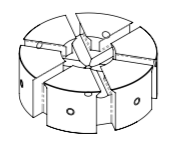
\includegraphics[width=0.3\textwidth]{Images/core}
   \caption{Core}
   \label{fig:core}
\end{figure} 

Cost is substantially driven by time; time to remove material in the machining process as well as set-up time of the machine itself\cite{SetUp}. Conveniently, our design is highly symmetrical meaning time and money is saved through lacking the need of a complex orienting mechanism given that the part's orientation prior to machining is irrelevant.

Finally, the volume of production is of great importance; with too small a batch size, set up costs and jig production costs become impractical and with too large a batch, storage costs pose a problem for a product of which the market response is not easily predictable. Considering the high cost and exclusive appeal of this product, low volume batch production in the order of 100 is appropriate so as to eliminate any unnecessary storage costs and allow adequate response to market needs. Specifically a volume of 300 pieces has been defined because it is divisible by three, the mounts are expected to be sold in groups of three, and during correspondence with Sylatech Ltd\textregistered it was discussed that any larger batch volume would pose an infeasible machining time; namely roughly two weeks.

\subsection{Secondary Processes}

A range of finishes best suited to individual parts have been chosen based on 
its functionality and location. A relatively cheap 2B (basic smooth) finish is 
to be applied to the stainless steel core so as to prohibit unnecessary 
expenditure considering the part shall not be seen by the customer whilst 
ensuring a path of minimal friction exists for the moving ball bearings. 
Additionally, the standard aluminium mill finish is rough and so all internal 
aluminium preloading pieces are to be brushed in the direction the piece 
travels so as to limit the amount of wear. Furthermore, the external retainer 
is to be brushed in concentric circles to give an attractive finish and hide 
any scratches. A 2J finish is to be applied to all other external stainless 
steel pieces as it is cheaper to produce than polishing and is practical in 
that it is resistant to scratches whilst being aesthetically 
pleasing\cite{Finishes}.\\

All parts are to be machined at fine linear and angular tolerances of +/-0.1mm 
and +/-$1\,^{\circ}\mathrm{}$ respectively to ensure the overall quality of the 
product. However there exists opportunity for optimisation within this section; 
in the interest of reducing cost, it was concluded that the rails contained in 
the core piece are the only parts to be machined to a high tolerance since they 
are to fit plush to the bearings; all other parts may be machined to a coarser, 
and therefore cheaper, tolerance.

\subsection{Manufacture Costs} \label{sec:ManCosts}
\subsubsection{Optimisation}
Sylatech Ltd\textregistered, a machining company situated in the North East of England, was contacted regarding the cost to manufacture the product and proved very informative with regard to the feasibility of our product. Initially a cost of roughly \textsterling500 per piece (for a batch volume of 300) was quoted which, allowing for appropriate margins detailed in section \ref{sec:Margins}, dictates a retail price of \textsterling1650. The most expensive existing product of similar concept is priced at \textsterling849.99 and, although our original product features merit a higher retail price, a difference of roughly \textsterling800 is too large when introducing a new product to the market. 

The following suggestions were made to reduce the quoted figure;
\begin{itemize}
    \item The rails of the core piece were to be modified such that the radius of the bearing race was continued until tangential with the wall. Simply, the right-angles depicted in Figure \ref{fig:RailCross} were to be removed. This revision was quoted to save roughly \textsterling100 per mount.
    \item The 0.3mm dimension of the base as shown in Figure \ref{fig:BaseCross} was to be extended to 2mm; the larger dimension is easier to grip and therefore would require less delicate and costly machine handling. This change was quoted to save roughly \textsterling10 per base.
    \item The retainer was to be machined using a 4 axis CNC machine which is considerably faster because fewer operations are required. This change was quoted to save roughly \textsterling20 per piece.
\end{itemize}


\begin{figure}[h]
   \centering
   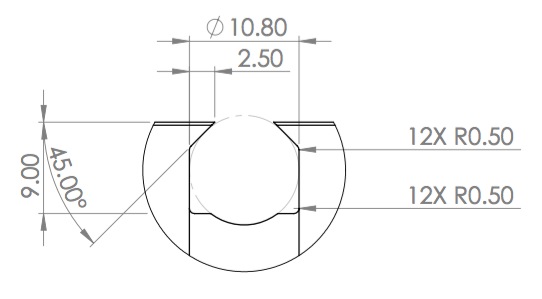
\includegraphics[width=0.5\textwidth]{Images/RailCrossSection}
   \caption{Bearing Race Cross Sectional Drawing}
   \label{fig:RailCross}
\end{figure} 

\begin{figure}[h]
   \centering
   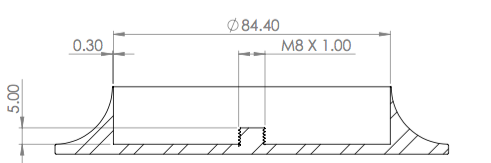
\includegraphics[width=0.5\textwidth]{Images/BaseCrossSection}
   \caption{Base Cross Sectional Drawing}
   \label{fig:BaseCross}
\end{figure} 

\subsubsection{Costing}

\begin{table}[H]
	\centering
	\footnotesize
	\begin{threeparttable}
	\caption{Costing}
        \label{table:costs}
	\begin{tabular}{@{}cp{9em}crr@{}}
		\toprule
		Item No. & Part No.  & Qty. & �/Piece & � Total \\
		\midrule
		1 & COR080-0003 & 1 & 97.00 & 97.00 \\
		2 & PLD080-0003  & 1 & 35.00 & 35.00 \\
		3 & PLD010-1004  & 6 & 2.00 & 12.00 \\
		4 & F669-N45SH-10 (first4magnets) & 12 & 0.30 & 3.60  \\
		5 & 10MMTUNGSTENB ALLS (VXB Bearings) & 6 & 20.30 & 121.80 \\
		6 & TOP080-0004A  & 1 & 32.50 & 32.50 \\
		7 & RET080-0003 & 1 & 25.00 & 25.00 \\
		8 & M4X20-CSK-ST (westfieldfasteners) & 6 & 0.09 & 0.54 \\
		9 & M4X20-CSK-H (westfieldfasteners) & 1 & 0.04 & 0.04 \\
		10 & USR080-0002 & 1 & 14.30 & 14.30 \\
		11 & RET080-1002  & 1 & 12.00 & 12.00 \\
		12 & USR080-1002 & 1 & 20.00 & 20.00 \\
		\bottomrule
		& & & & 373.78\tnote{1}
\end{tabular}
  \begin{tablenotes}
            \raggedright
            \tiny
            \item[1]{Sylatech Ltd, Kirkdale Road, Kirkbymoorside, North Yorkshire, YO62 6PX, Quote courtesy of Mr R McGill}
        \end{tablenotes}
    \end{threeparttable}
\end{table}
Table \ref{table:costs} details the final cost of off-the-shelf parts and machining 
per mount, totalling 393.78 per mount.

\section{Design for Assembly} 
\subsection{Jig Design}
Due to the small scale of our product, hand assembly is required. Considering the complexity of the design and physical impracticality of overcoming the repulsive magnetic forces during its assembly, a jig has been designed, as shown in drawings JIG080-0001 and JIG080-1001, with full accompanying assembly instructions (see Isofonics Assembly Instructions ISO080-INS).

\begin{figure}[h]
    \centering
    \subfloat[Assembly Jig Base] 
        {{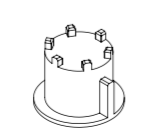
\includegraphics[width=0.4\textwidth]{Images/jigbase} }}%
    \qquad
    \subfloat[Assembly Jig Sleeve] 
        {{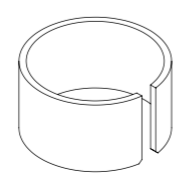
\includegraphics[width=0.3\textwidth]{Images/jigsleeve} }}%
    \caption{Assembly Jig Components}
    \label{fig:JigAssembly}
\end{figure}

\subsection{Assembly Costs} \label{sec:AssemCosts}
Considering the assembly jig is to be re-used indefinitely, its cost is negligible within the context of the product's assembly. Assembly costs are then only defined by the time taken to manually assemble the device and the cost of manual labour which can be estimated at 2 minutes and \textsterling8/hr respectively. This equates to a total of \textsterling0.27 per piece.

\section{Design for Sustainability}
Isofonics recognises the importance of considering the environmental implications of the manufacture as well as disposal of any product.

Isofonics footers are made to last a lifetime. This is achieved by using the highest quality materials possible; quality and endurance were more important than the price of the product considering the high budget of the design. This reduces the harm done to the environment by
eliminating the need to manufacture replacement footers.Another method of ensuring minimal impact is to reduce the scrap, this is
achieved by ensuring that the size of the raw material is a similar size to the final product. The main central section of the footer is produced using a CNC machining process as described previously and so the un-refined steel will be cut to within a small tolerance of the final product. The scrap that is inevitably produced will be recycled; this includes both stainless steel and aluminium.\\

Stainless steel contains valuable raw materials, especially chromium, nickel and molybdenum and hence recycling it is economically viable. Like many other metallic materials, stainless steel is recycled through a re-melting process, where the melted steel is re moulded for use. Similarly, aluminium is also recycled with a re-melting process and can be reprocessed and reformed endlessly without losing any of its quality.\\

Packaging often contributes to the waste generated by the product; to avoid this, the footers will be packaged in simplistic cardboard based materials which can be efficiently recycled rather than plastics where the recycling process yields less useful products.


\section{Commercial Considerations} 

\subsection{Brand Development and Competitor Analysis}
With the intention of establishing the design in the market, a brand identity 
was essential. Through several brainstorming sessions, the team agreed on the 
name \textquotesingle Isofonics \textquotesingle.\\

It was important to review the current market leaders, 
Stillpoints and Nordost, with their relevant products. Nordost primarily 
manufactures Hi-Fi audio cables but recently introduced additional products for 
resonance and power control. Namely, their \textquotesingle SortKone\textquotesingle acts as a vibration 
drain with a mechanical diode effect to prevent external vibrations from 
travelling up through the cone. Similarly, 3 cones are recommended per device 
but they offer 3 types of cone, each made from different materials. The most 
expensive is made from titanium and utilises ceramic bearings, retailing at 
\textsterling349.99 per cone.\cite{Nordostcost} Stillpoints offer an equivalent solution, their most expensive is their ?Ultra 6,? priced at \textsterling799.99 per mount and \textsterling849.99 with an accompanying base. \cite{StillpointsCost}
 
\subsection{Stillpoints Patent Check}
 
Stillpoints\textquotesingle patent for their \textquotesingle Universal Vibration Damper\textquotesingle was thoroughly studied and the potential risks of infringement were identified. Their patent details the design of a \textquotesingle device for the control of vibrations comprising a retainer resting on a base and a plurality of bearings disposed within the retainer.\textquotesingle  It focuses mainly on the use of layered bearings and springs to diminish the signals through friction with three or more on the first layer and at least a substantially larger one on the second. Each bearing on the first layer is held by the base plate and side of the retainer and supports the bearing above. It also explores other options to replace the springs such as using opposing magnets: \textquotesingle In some embodiments the first base member 119 and second base member 123 may have opposing magnetics fields.\textquotesingle \cite{Stillpoints} However, Isofonics? product is not an embodiment of the mechanism described in the first claim of the patent. A cone with a retaining flange is used rather than the layers of spherical bearings.
 
\subsubsection{Parallels with Stillpoints}
The following details the main claim made by Stillpoints and highlights areas 
of concern:

\lq{A device for the control of vibrations comprising:
\emph{a retainer}, the retainer constructed and arranged to rest upon a base, at least a \emph{portion of the base defining a substantially flat surface}; and \emph{a plurality of bearings disposed within the retainer, the bearings arranged in a first layer and a second layer}, the second layer disposed on the first layer, the first layer comprising three or more bearings, and the second layer comprising at least one bearing, each bearing in the first layer constrained on its bottom by only the substantially flat surface of the base, on its side by the retainer, the bearings in the first layer supporting the at least one bearing in the second layer, the retainer defining a surface which is in substantially tangential contact with the bearings in the first layer}\rq\cite{Stillpoints}.\\

It is clear that the main claim focuses on the use of layers of bearings, in this way, our design is fundamentally different. Since our design differs from that outlined in the main claim, all further claims based on the first are irrelevant. An element of originality of our design lies in the use of magnets which is not mentioned at all within the official claims section of the patent.

\begin{figure}[H]
    \centering
    \subfloat[Stillpoints Mechanism Diagram]
        {{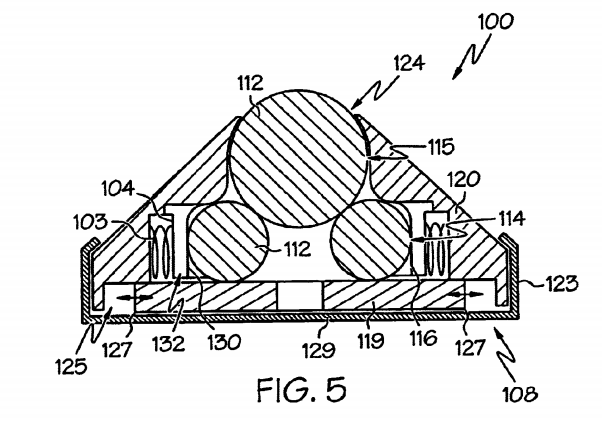
\includegraphics[width=0.4\textwidth]{Images/Stillpoints} }}%
    \qquad
    \subfloat[Group 25 Mechanism Diagram]
        {{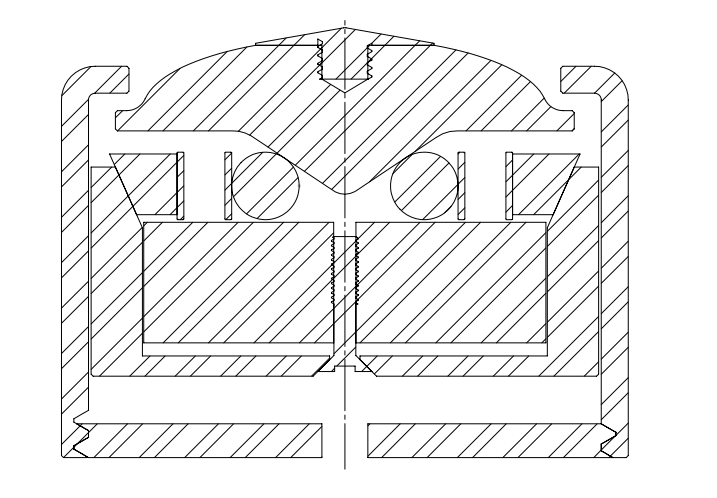
\includegraphics[width=0.4\textwidth]{Images/Group25} }}%
    \caption{Stillpoints Mechanism Comparison}
    \label{fig:Patent}
\end{figure}

To verify that the mounts did not bear a resemblance to Stillpoints\textquotesingle invention, Robin Bartle, a patent lawyer from Bartle Read, a company based in Liverpool which specialise in intellectual property was contacted who was able to confirm that \textquotesingle Because the mount does not feature a second layer of bearings as shown on the cross-section, there are no blatant overlaps between the two products and Stillpoints would not have sufficient grounds to sue\textquotesingle (see Figure \ref{fig:Patent}). Additionally, Mr Bartle noted that this is a US patent and is not filed with the European Patent Office and so only stands to limit sales within the US.


\subsubsection{Points of Originality}
\begin{itemize}
    \item Use of \emph{opposing magnetic fields} for lateral damping as 
    opposed to springs
    \item \emph{Cone with retaining flange} replacing layers of bearings
    \item \emph{Pre-loading mechanism} in which a screw in tension moves a 
    fixed magnet decreasing its distance from the bearing magnet thus 
    increasing the strength of the system---adjustable for a variety of masses.
\end{itemize}

\subsection{Marginal Costs} \label{sec:Margins}
With reference to Table \ref{table:costs}, and accounting for assembly costs as discussed in section \ref{sec:AssemCosts}, the main contained mechanism, optional base and spike are to cost roughly \textsterling340 , \textsterling20 and \textsterling14.30 respectively to produce.
With respect to production costs, margins of 100\% for product distribution, 100\% for retail and 30\% for profit are to be met which consequently dictate the following retail prices. The main device shall retail for \textsterling1,149.00, the optional base for \textsterling66.00 and the removable spike for \textsterling49.00.

\section{Discussion} 
\subsection{Specification Fulfilment}
\subsubsection{User Requirement Specification Tree}

\emph {Eliminate Microphonic Effects}

The requirement for a rigid load path was integral to the performance of the damping mechanism. The interaction
between the magnets and the spherical bearings in conjunction with the hardness of their material diminished the excess mechanical vibrations generated by microphonic effects as demonstrated by the graphs produced by the
dynamic model. However, the data yielded during the experiment which was then inputted to the simulation, did not fully reflect the execution of the design and is therefore a source of uncertainty. Employing the squash balls as a method of dampening the noise produced by the amp did validate the concept but would be of more value if a prototype was used to establish a value empirically.

\emph {Budget Constraints}

With reference to the commercial considerations section and design for manufacture, it is clear that the market for
isolation devices is not driven by cost, instead by sound engineering science. However, in comparison with the
products introduced by Nordost and Stillpoints, the cost for one mount differs substantially and so must be justified.
For example, there is a \textsterling300 difference with Stillpoints Ultra 6 mount with the original costings. The advantages over these competitors are as follows:

\begin{itemize}
	\item Provide proof of concept through dynamic model.
	\item Appeal to hobbyists through hands-on \textquotesingle tweaking \textquotesingle graphs.
	\item One set of mounts accommodates a range of masses. More do not need to be bought for heavier/lighter devices, unlike with Stillpoints. 
	\item Use of premium materials, namely tungsten carbide bearings.
	\item M8 threads at the top and bottom pieces allow the user to amenably couple their device to the footers. 
\end{itemize}

\emph {Integrate with existing equipment}

The HiFi equipment must only rest on 3 footers to prevent further resonances and heating in the arrangement. If
another was used, it would either prove redundant or induce further noise. The cone provided a single point of contact which in turn meant that 3 footers were needed to support one piece of equipment. Partnered with the large base plate, this guaranteed that the mounts would not slip and the system was amply stable.
In addition, the aesthetically pleasing finishings ensure that the footer is well integrated with the existing system and is resistant to scratches. On the other hand, it could not be proven that the mount \textquotesingle avoids blemishing\textquotesingle because a prototype was not made and tested over a sufficient amount of time.

\subsection{Further Developments}
In the interest of expanding the design, a number of proposals have been made;

\begin{itemize}
\item Product families could be made, of differing size and/or material composition, to cater for an even wider range of masses to include heavier systems such as Loudspeakers.
\item A companion phone application which enables the user to adjust the preload for a desired condition could also replace the preloading graphs provided by the parametric model. 
\end{itemize}


Additionally, within this project exists great potential for further work to improve the design.

-3D modelling as opposed to 2d
-A 2-D finite element analysis software was used to model the magnetic flux distribution within the mount a 3-D software would have been preferable to more accurately determine...


\section{Conclusion}
The following statements summarise the main results of the project:
\begin{itemize}
	\item The URS tree provided a sound and comprehensive depiction of the brief.
	\item Suitable engineering techniques were applied. Namely, 2D finite element analysis and modelling the footer as a mass-spring system in Simulink.
	\item There were numerous revisions of the initial concept. For example, the addition of the cone, dome and M8 thread on the top piece. 
	\item The manufacturing considerations were detailed and were modified several times following feedback that some parts were too expensive or complex to machine. 
	\item A prototype must be made and tested to provide additional proof of concept and hence further justify the larger cost of the footer.
\end{itemize}

 In conclusion, it is clear that the final product met the initial design brief through the fulfilment of the greater part of the URS tree constructed in the feasibility report.




\section{References}
\printbibliography

% Appendicies
\clearpage
\appendix
\section{Project Plan and Members' Contributions} 
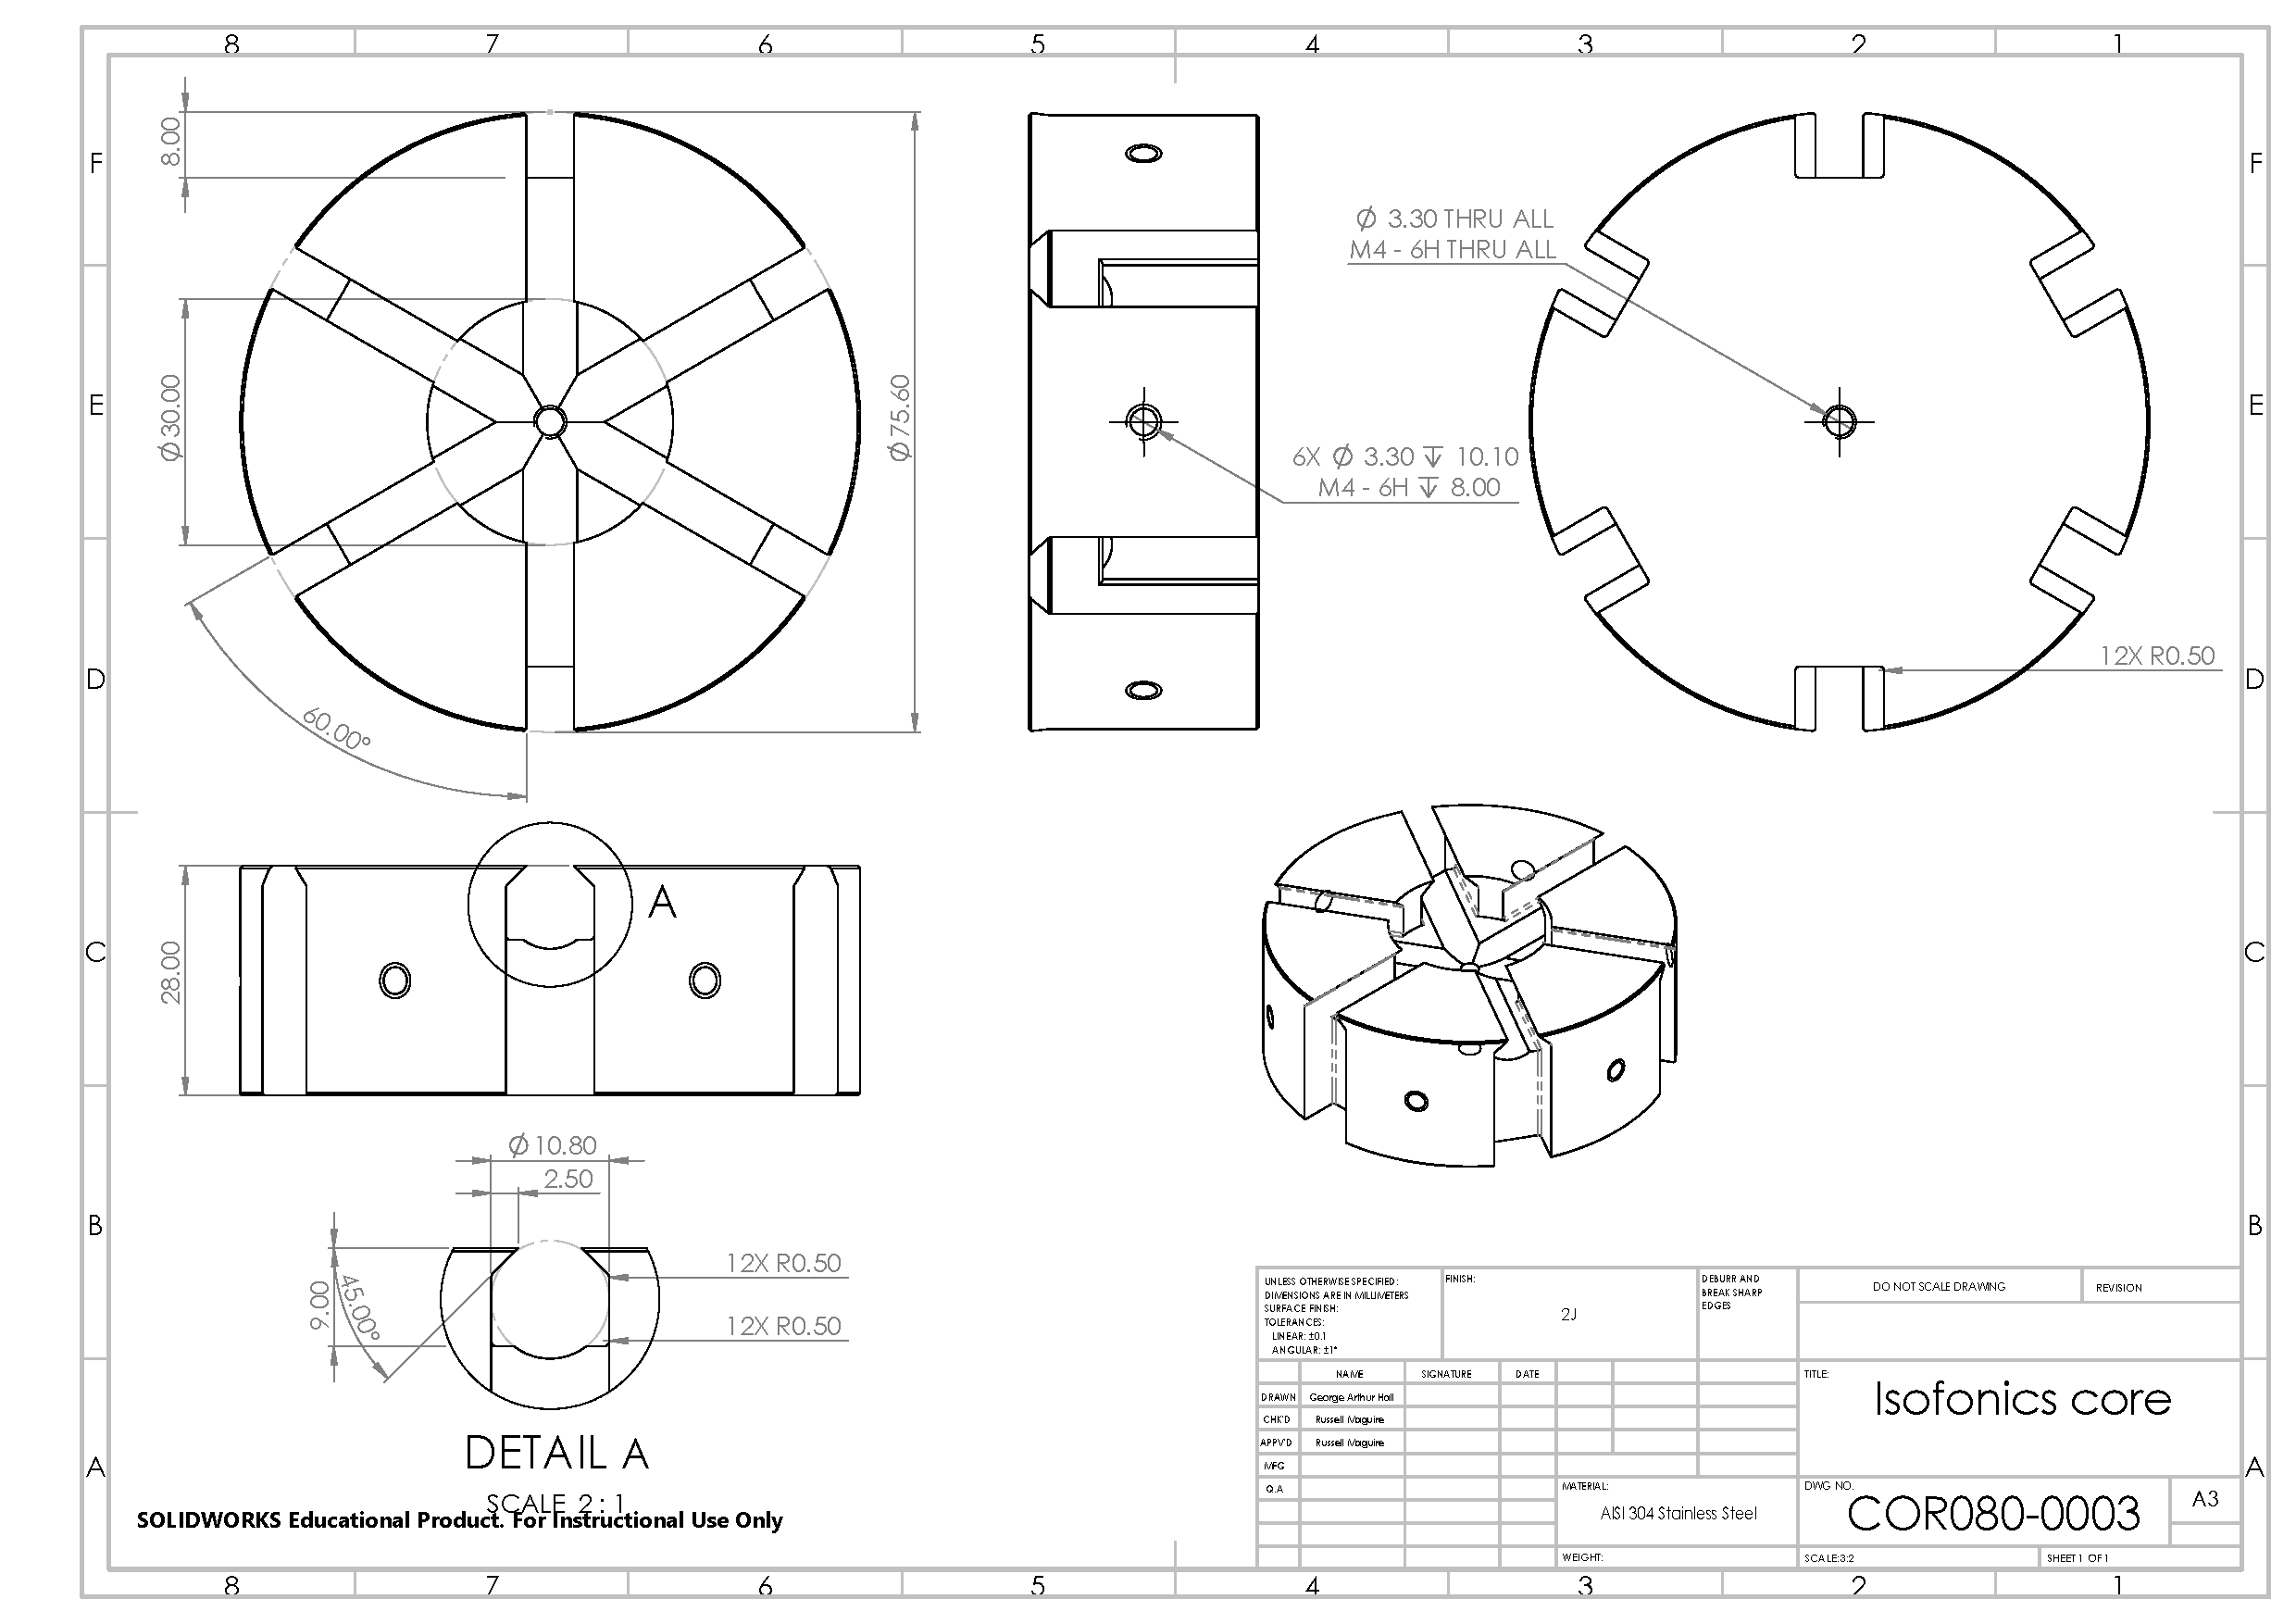
\includepdf[pages=-,fitpaper=true]{Images/Drawings/COR080-0003.PDF}
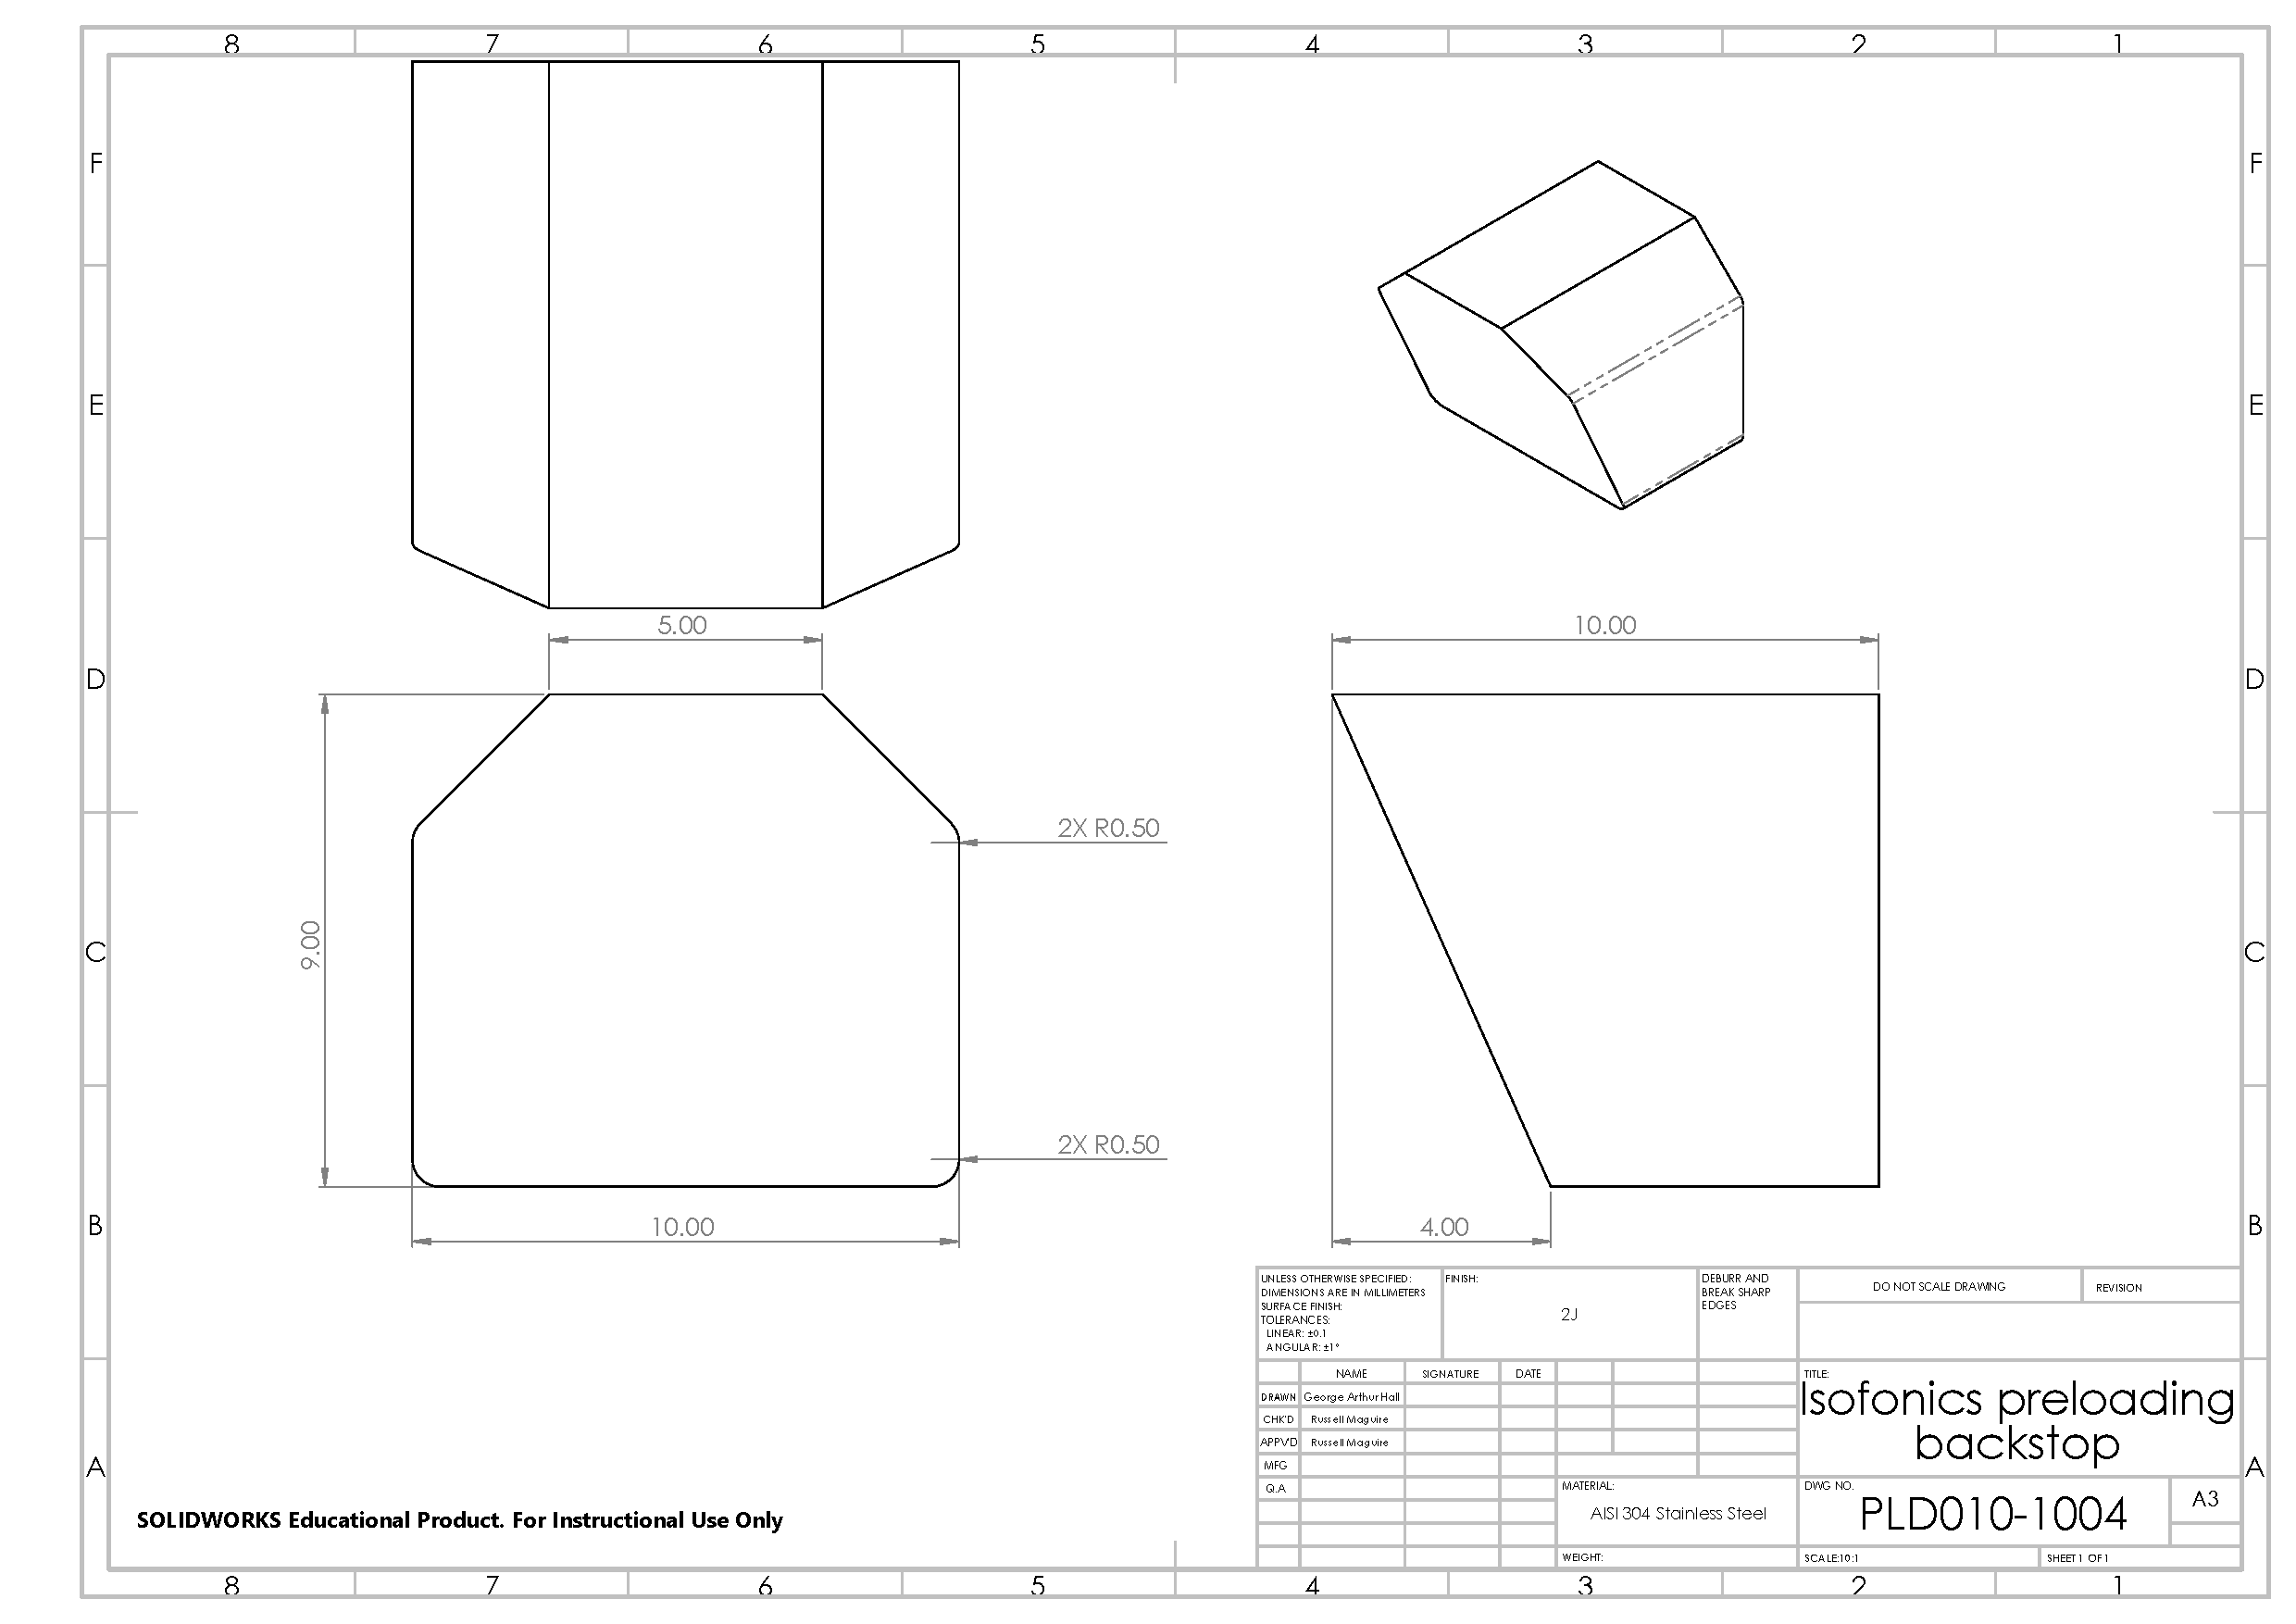
\includepdf[pages=-,fitpaper=true]{Images/Drawings/PLD010-1004.PDF}
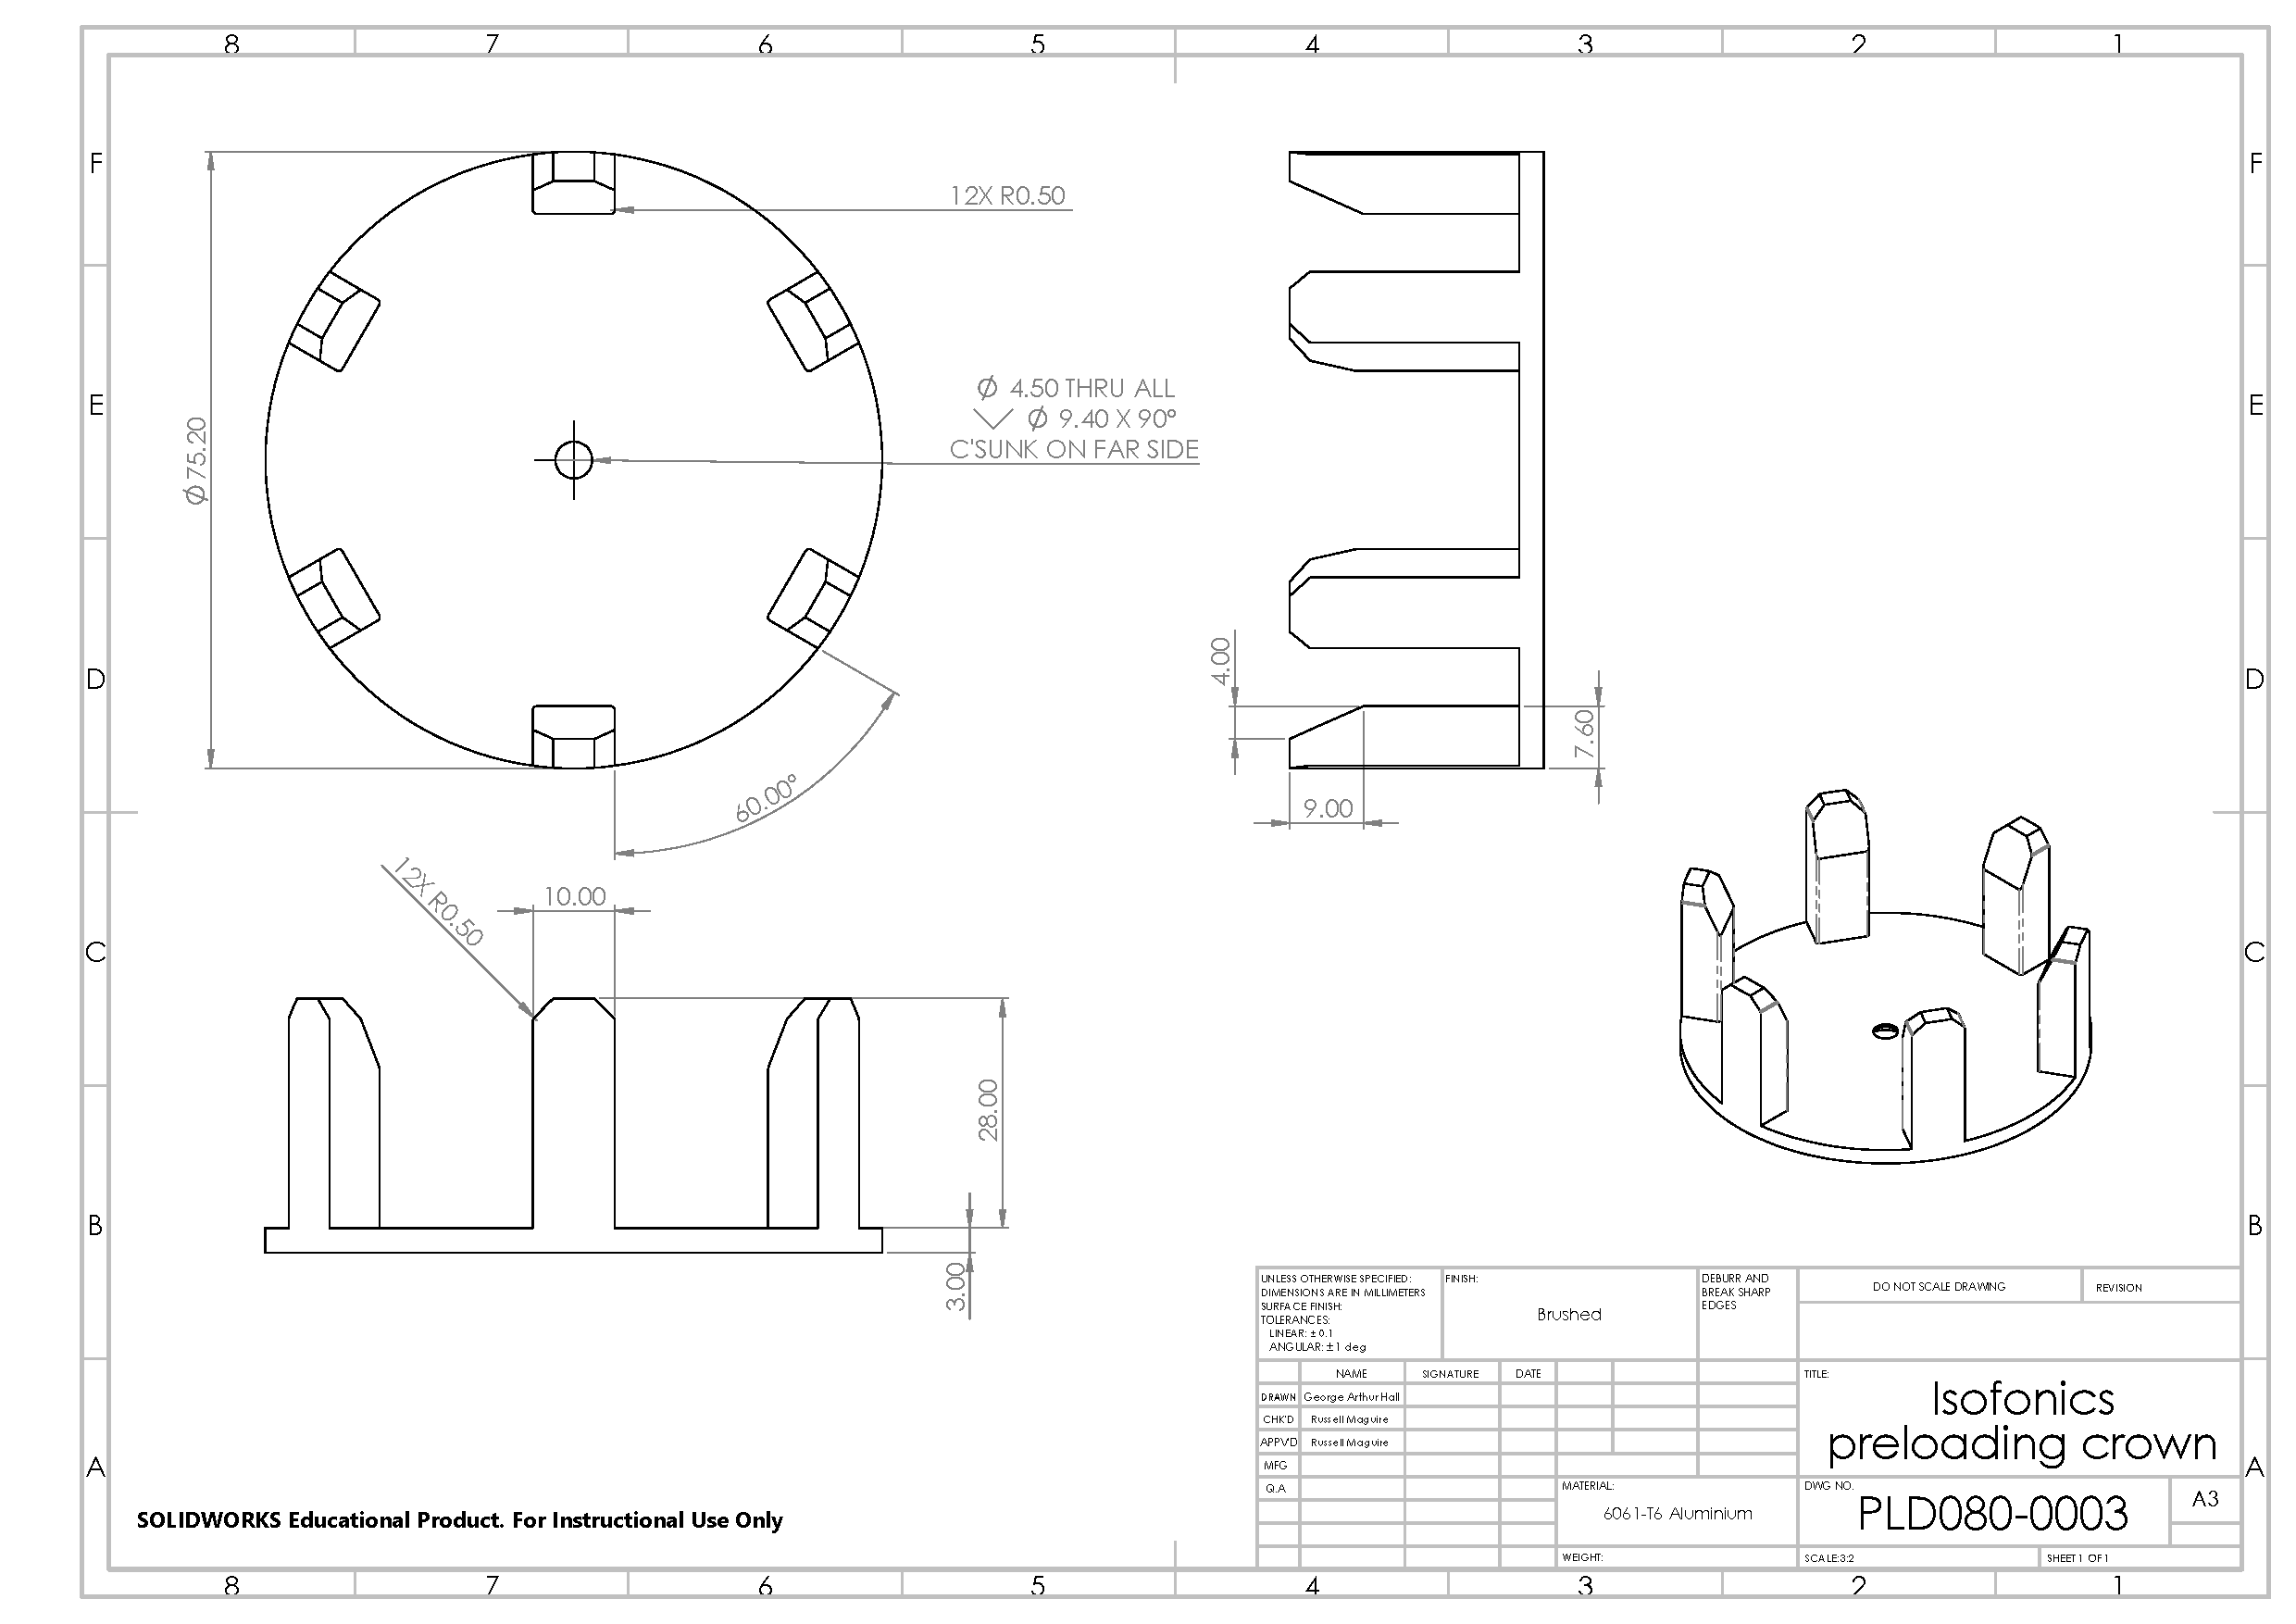
\includepdf[pages=-,fitpaper=true]{Images/Drawings/PLD080-0003.PDF}
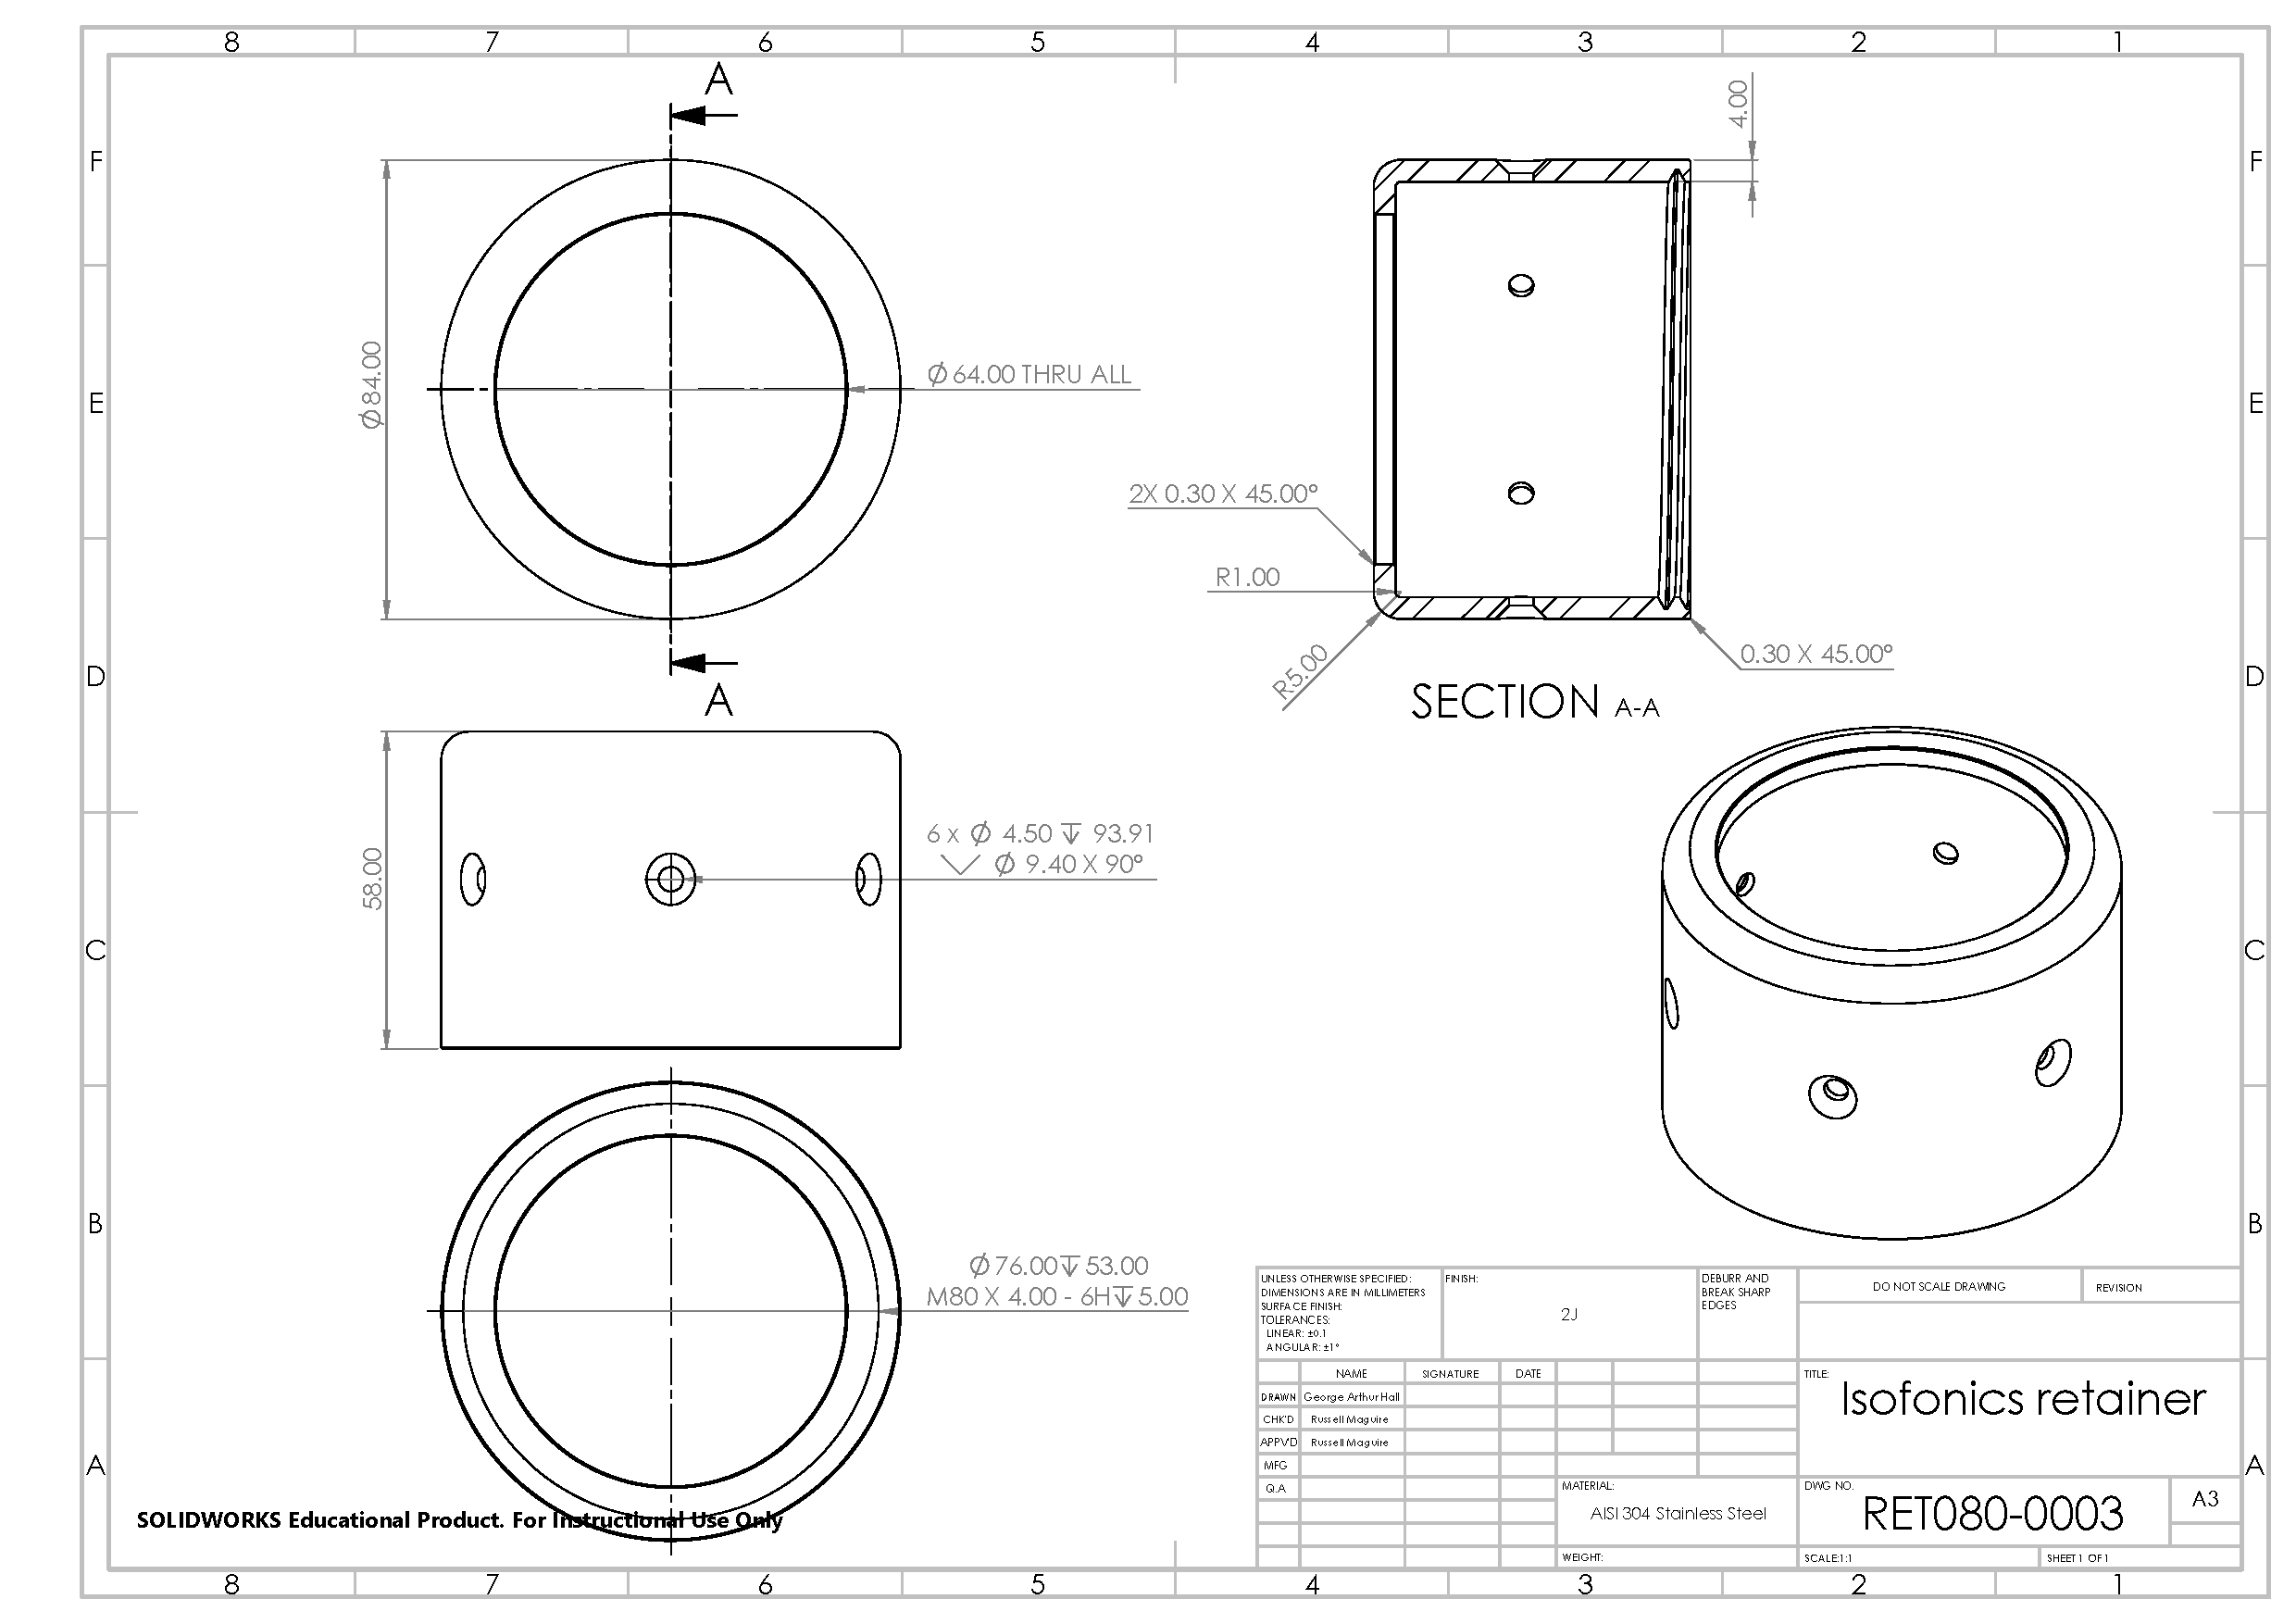
\includepdf[pages=-,fitpaper=true]{Images/Drawings/RET080-0003.PDF}
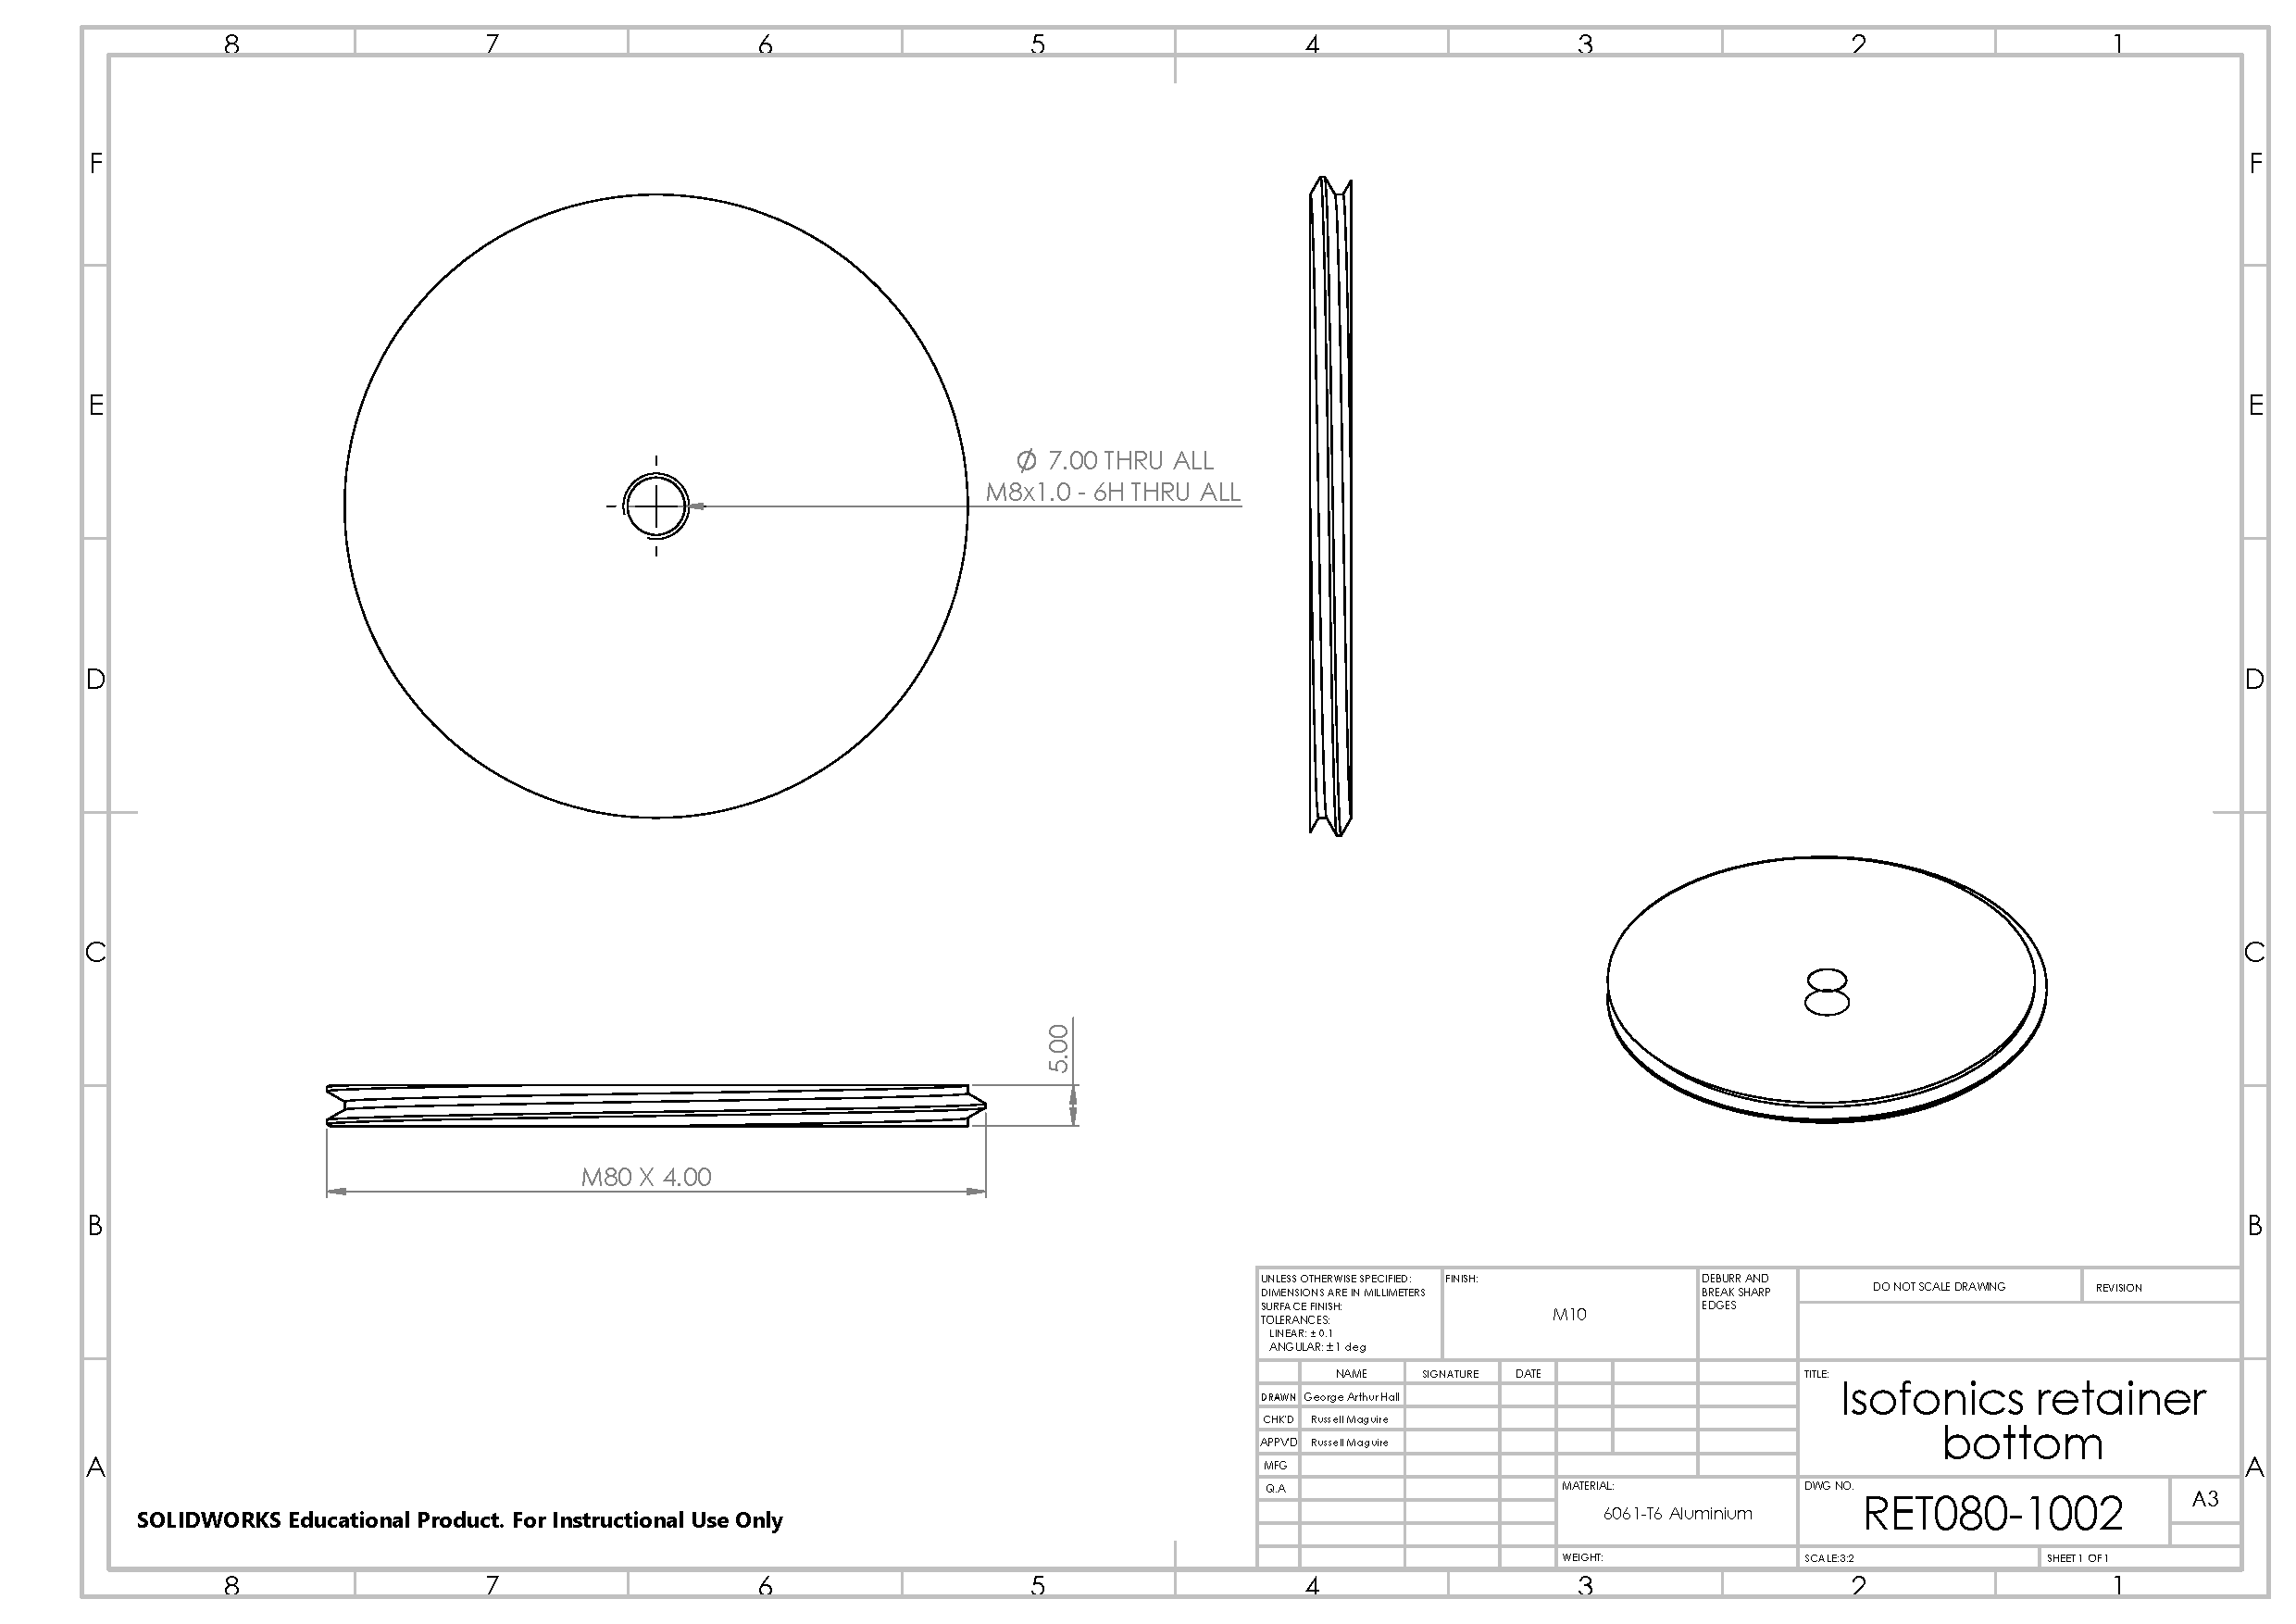
\includepdf[pages=-,fitpaper=true]{Images/Drawings/RET080-1002.PDF}
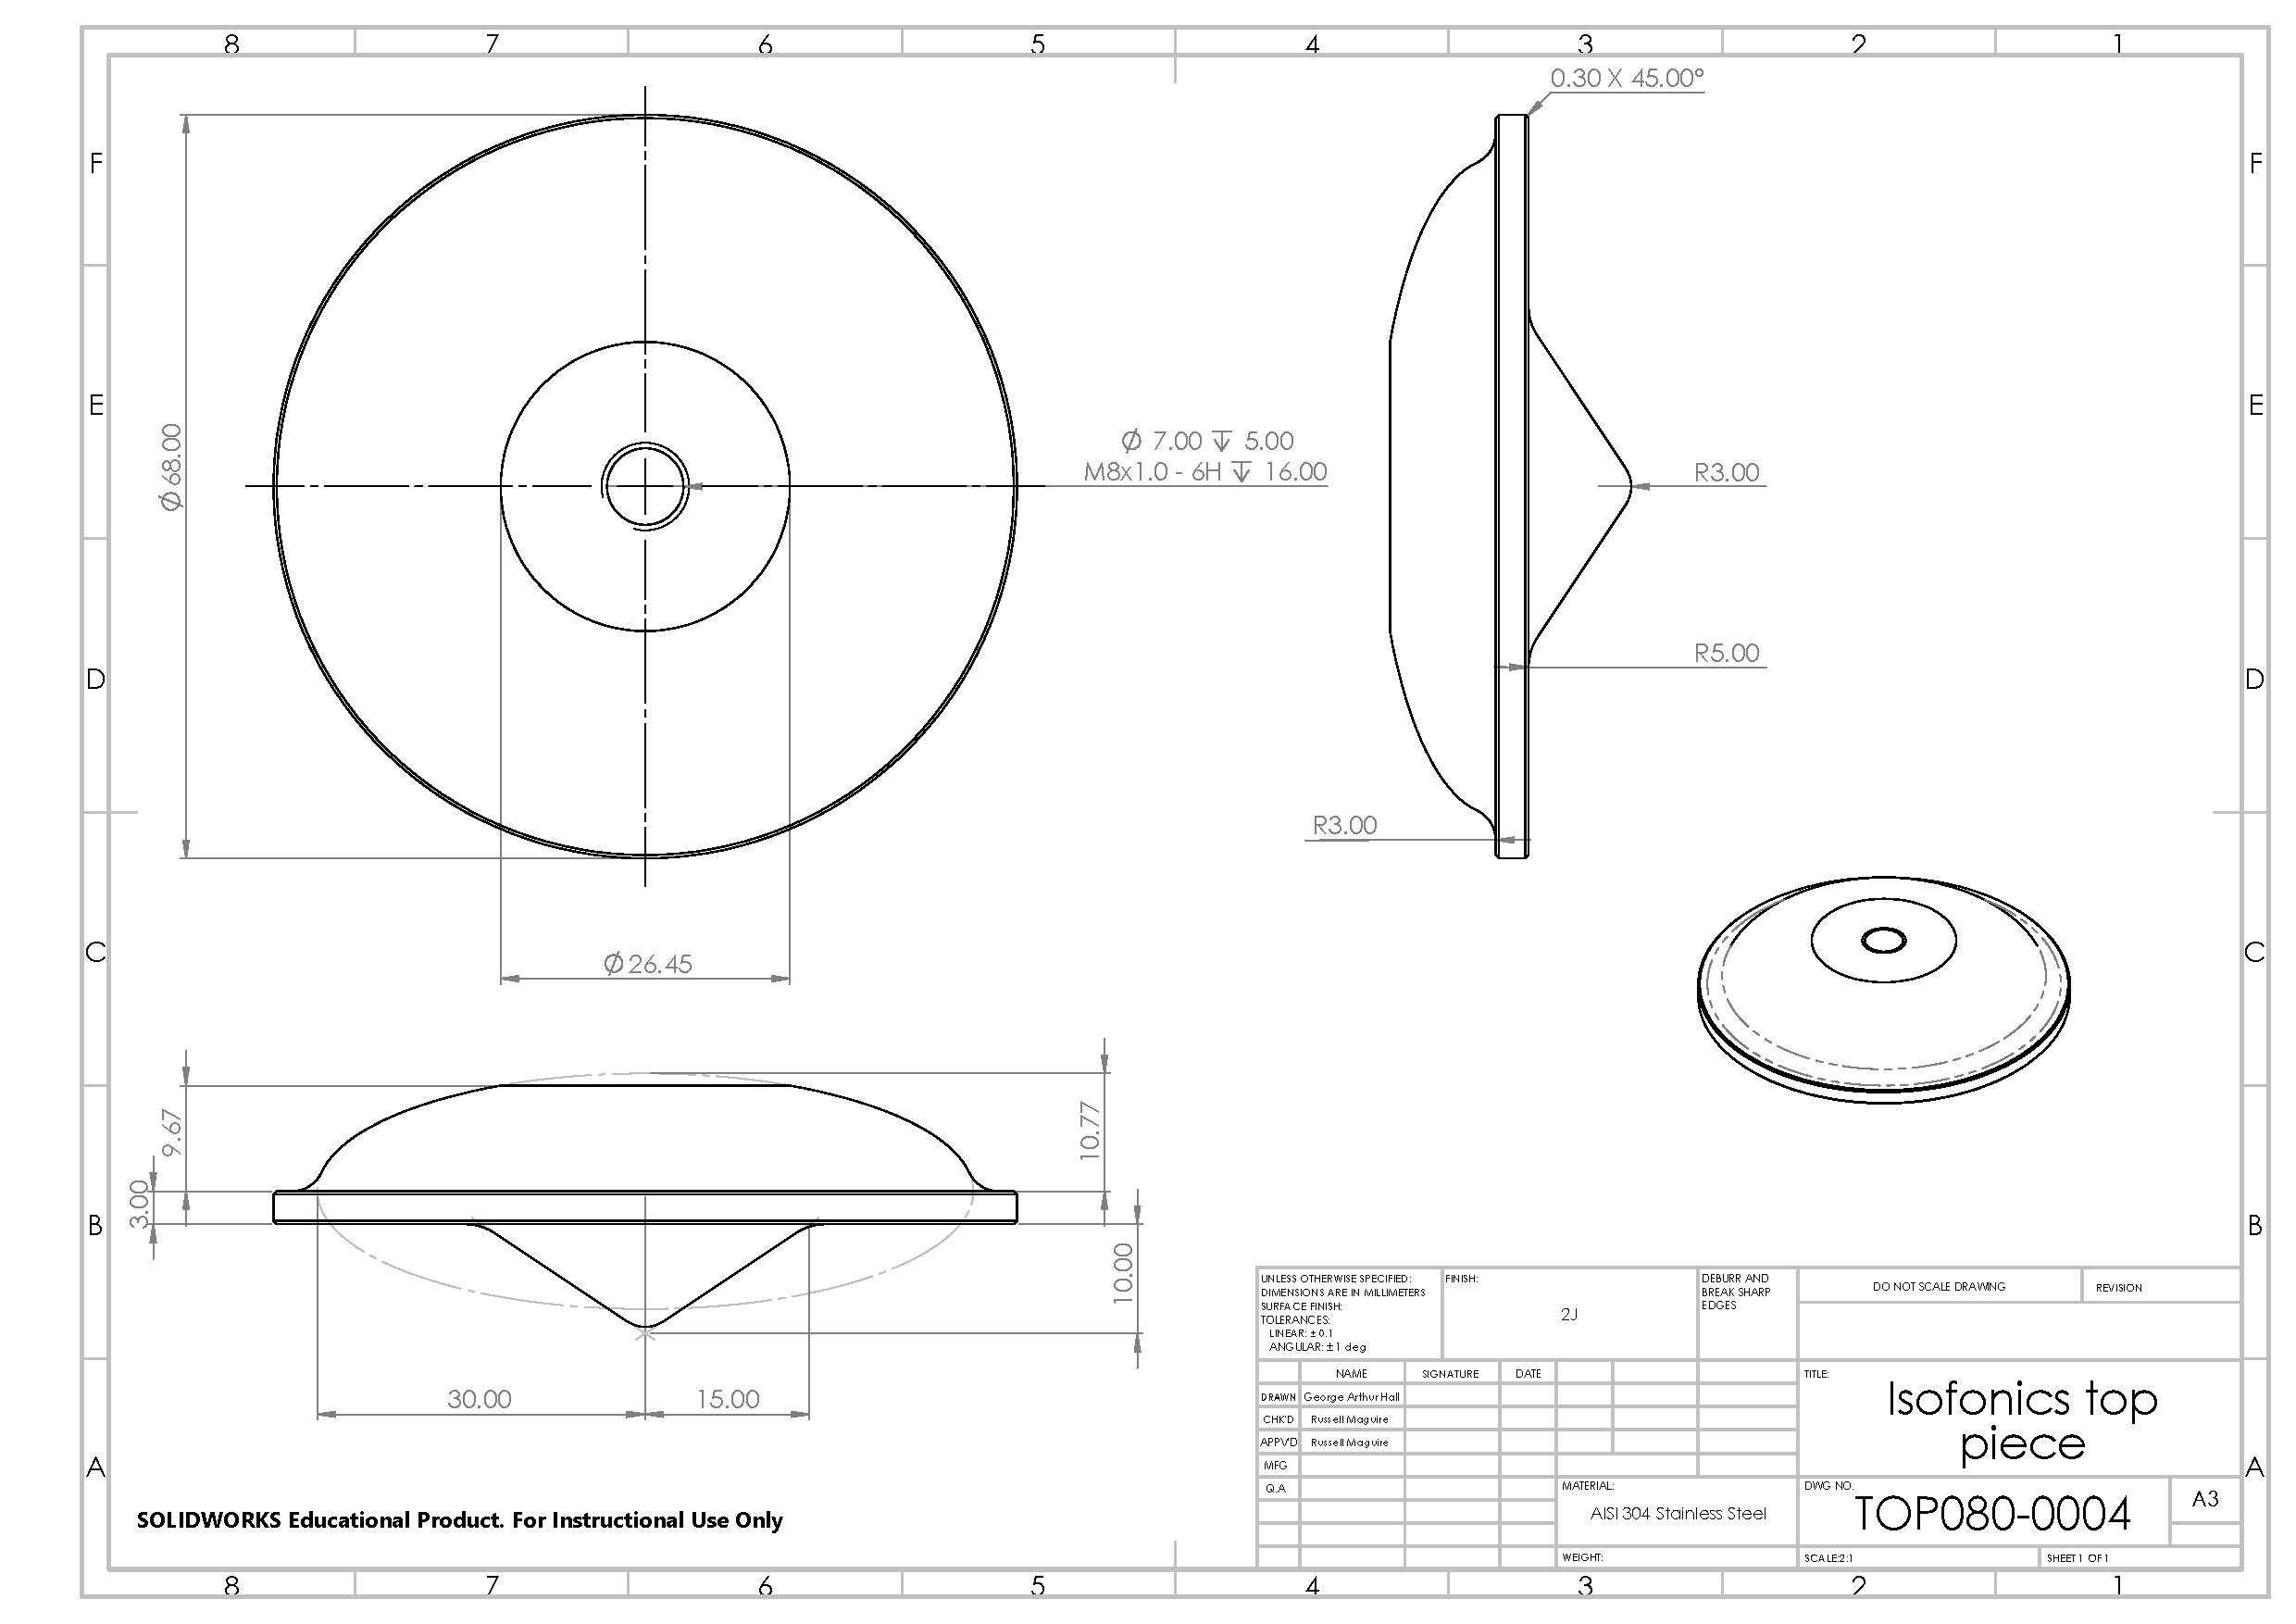
\includepdf[pages=-,fitpaper=true]{Images/Drawings/TOP080-0004.PDF}
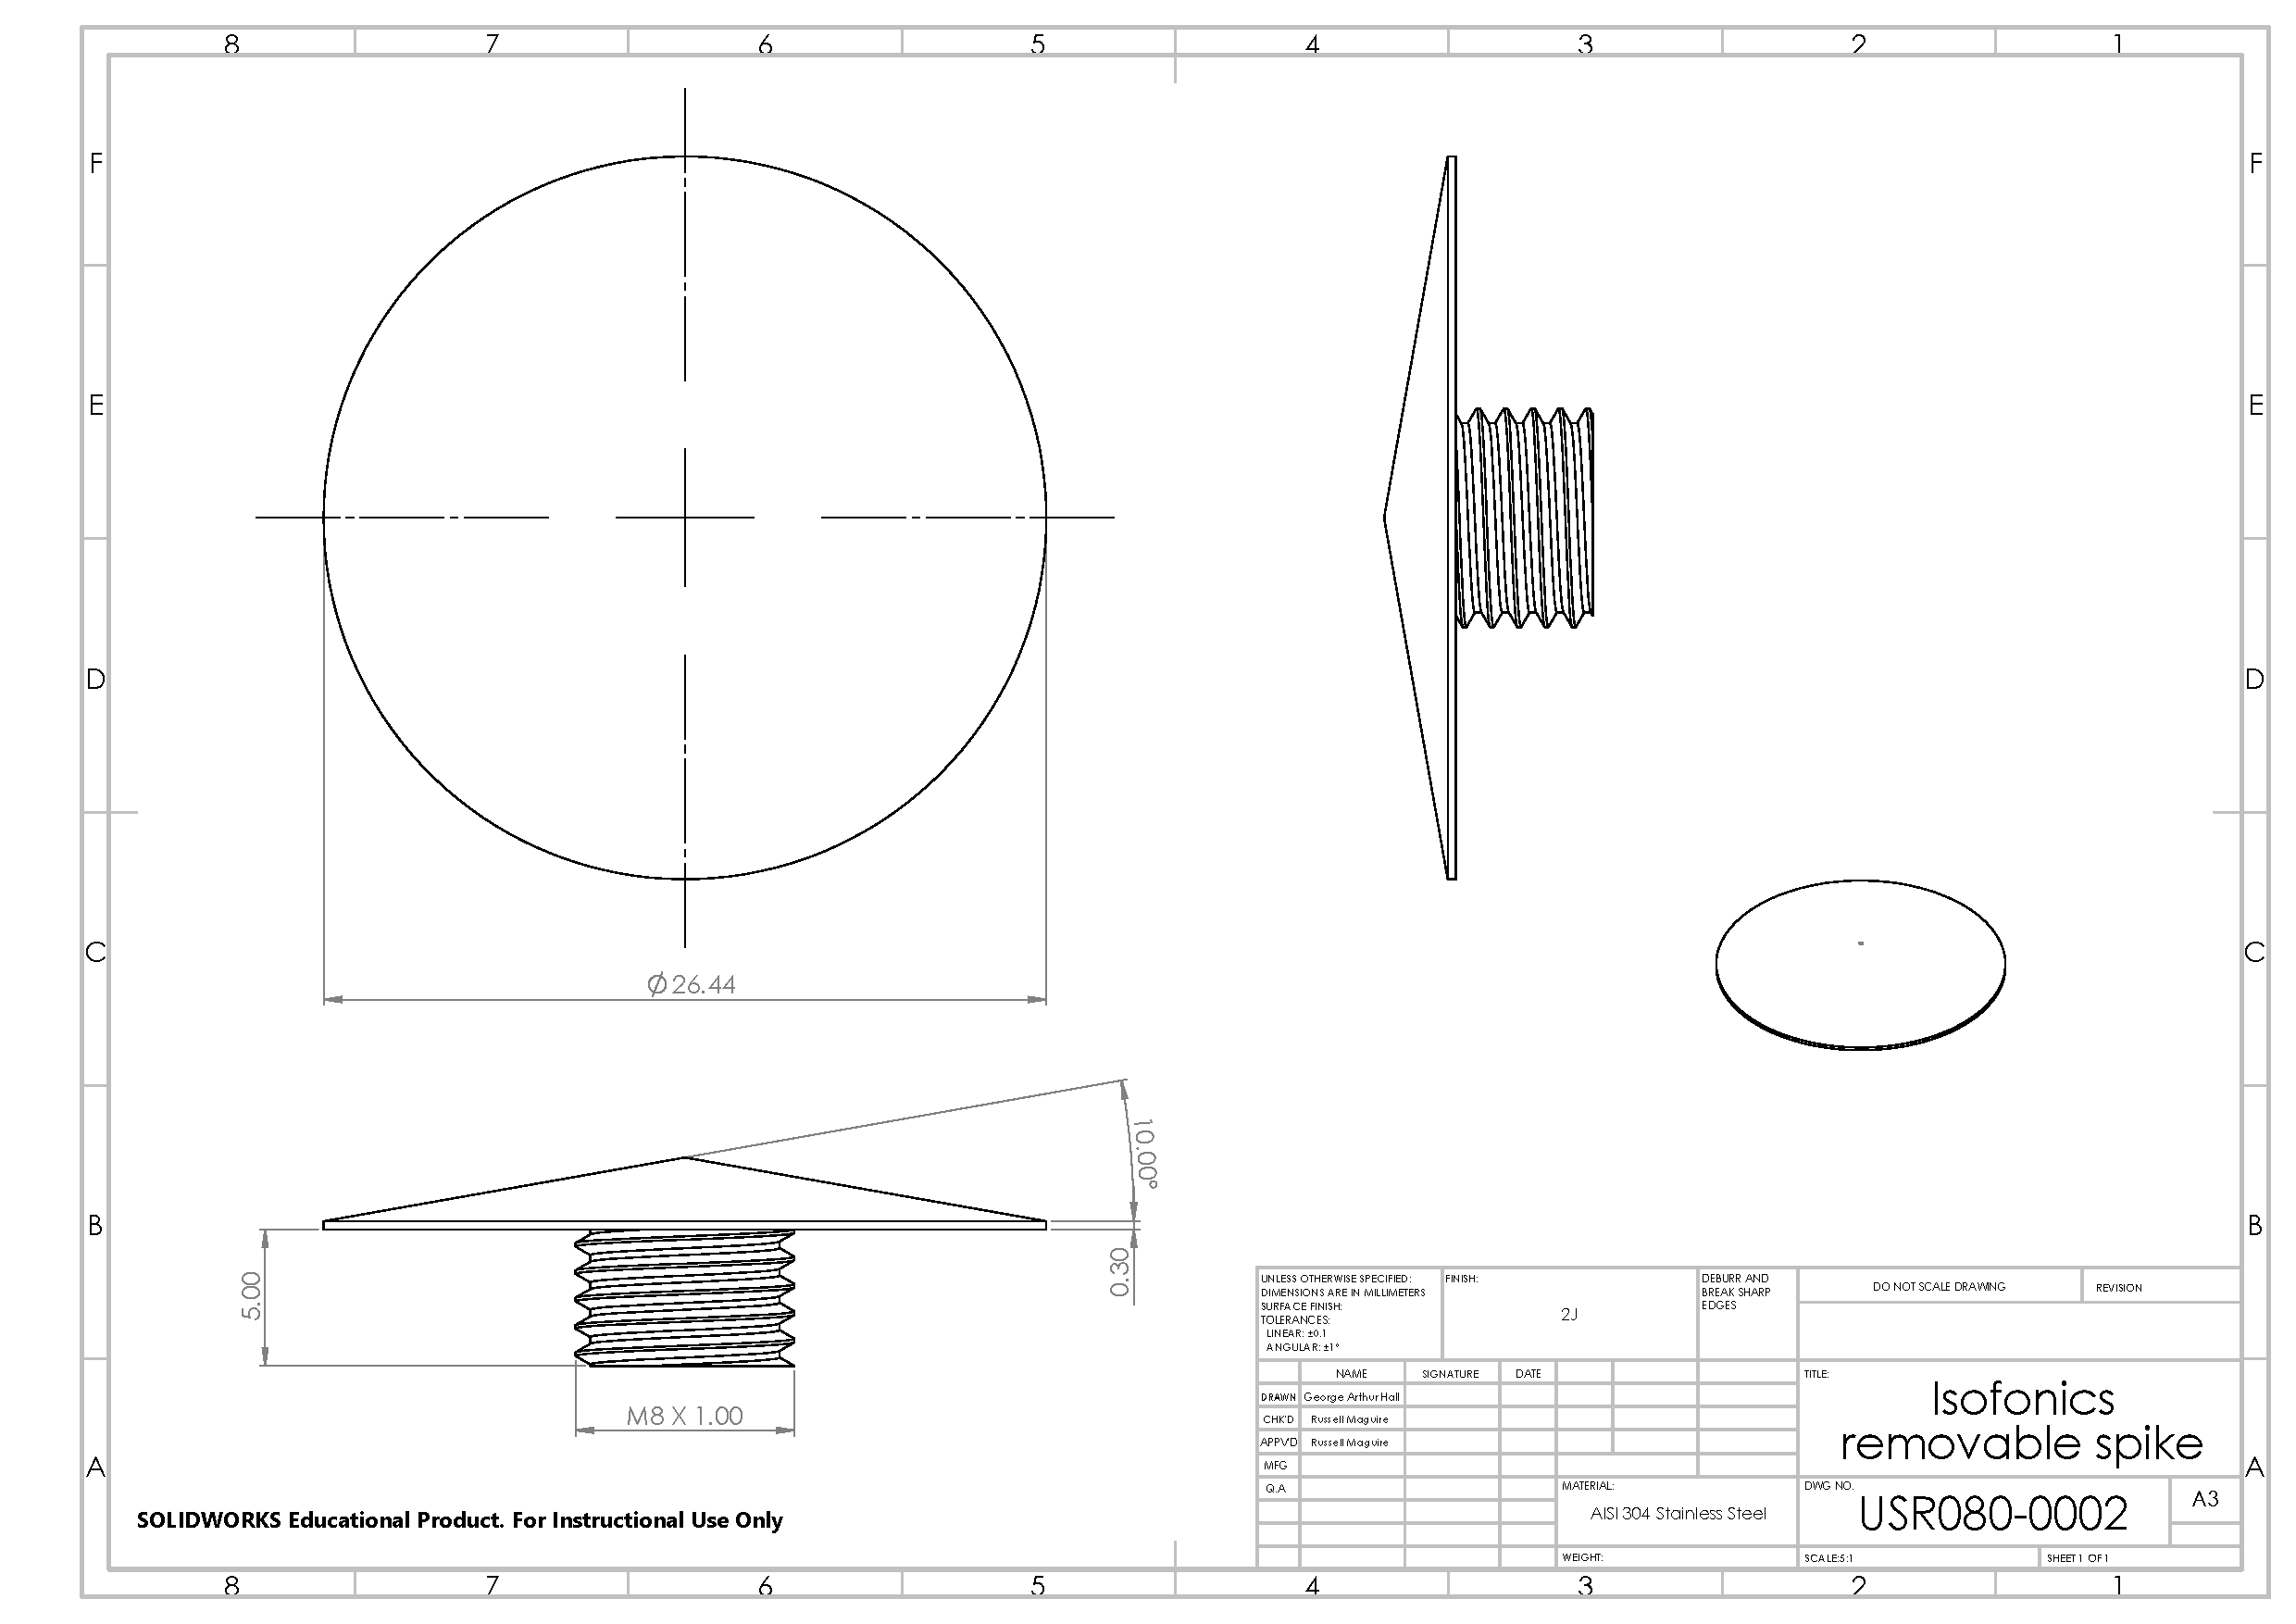
\includepdf[pages=-,fitpaper=true]{Images/Drawings/USR080-0002.PDF}
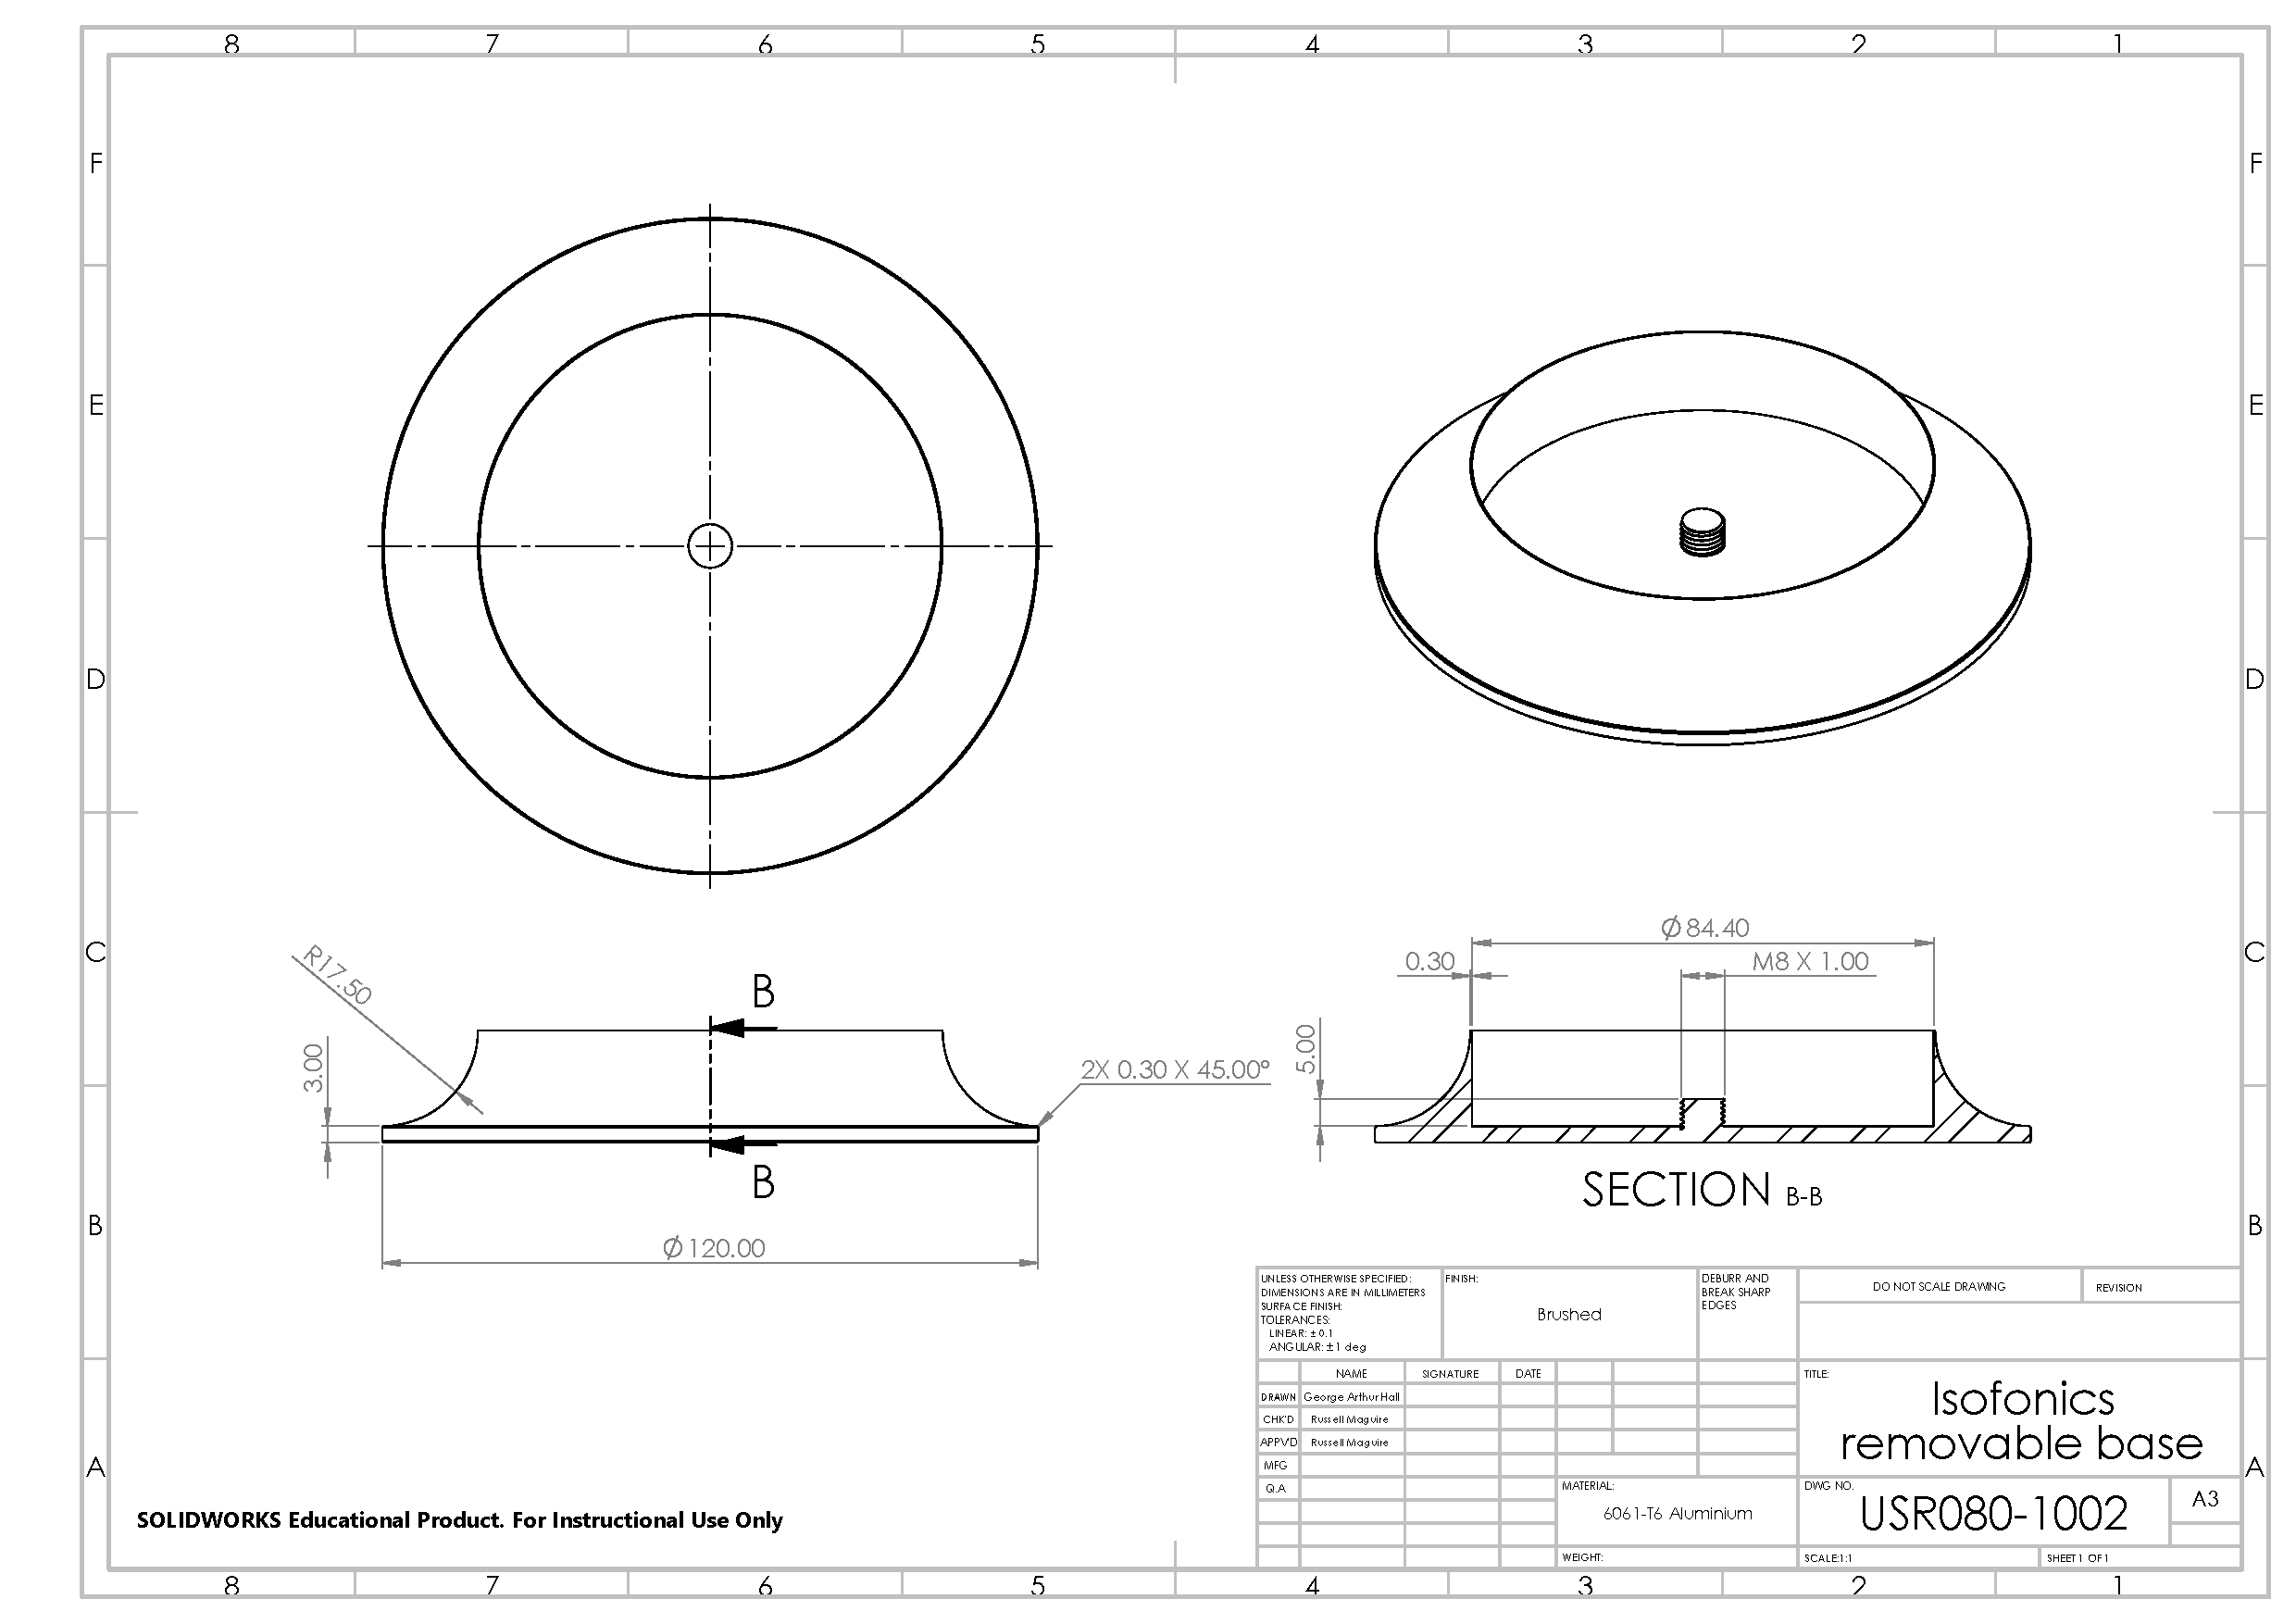
\includepdf[pages=-,fitpaper=true]{Images/Drawings/USR080-1002.PDF}

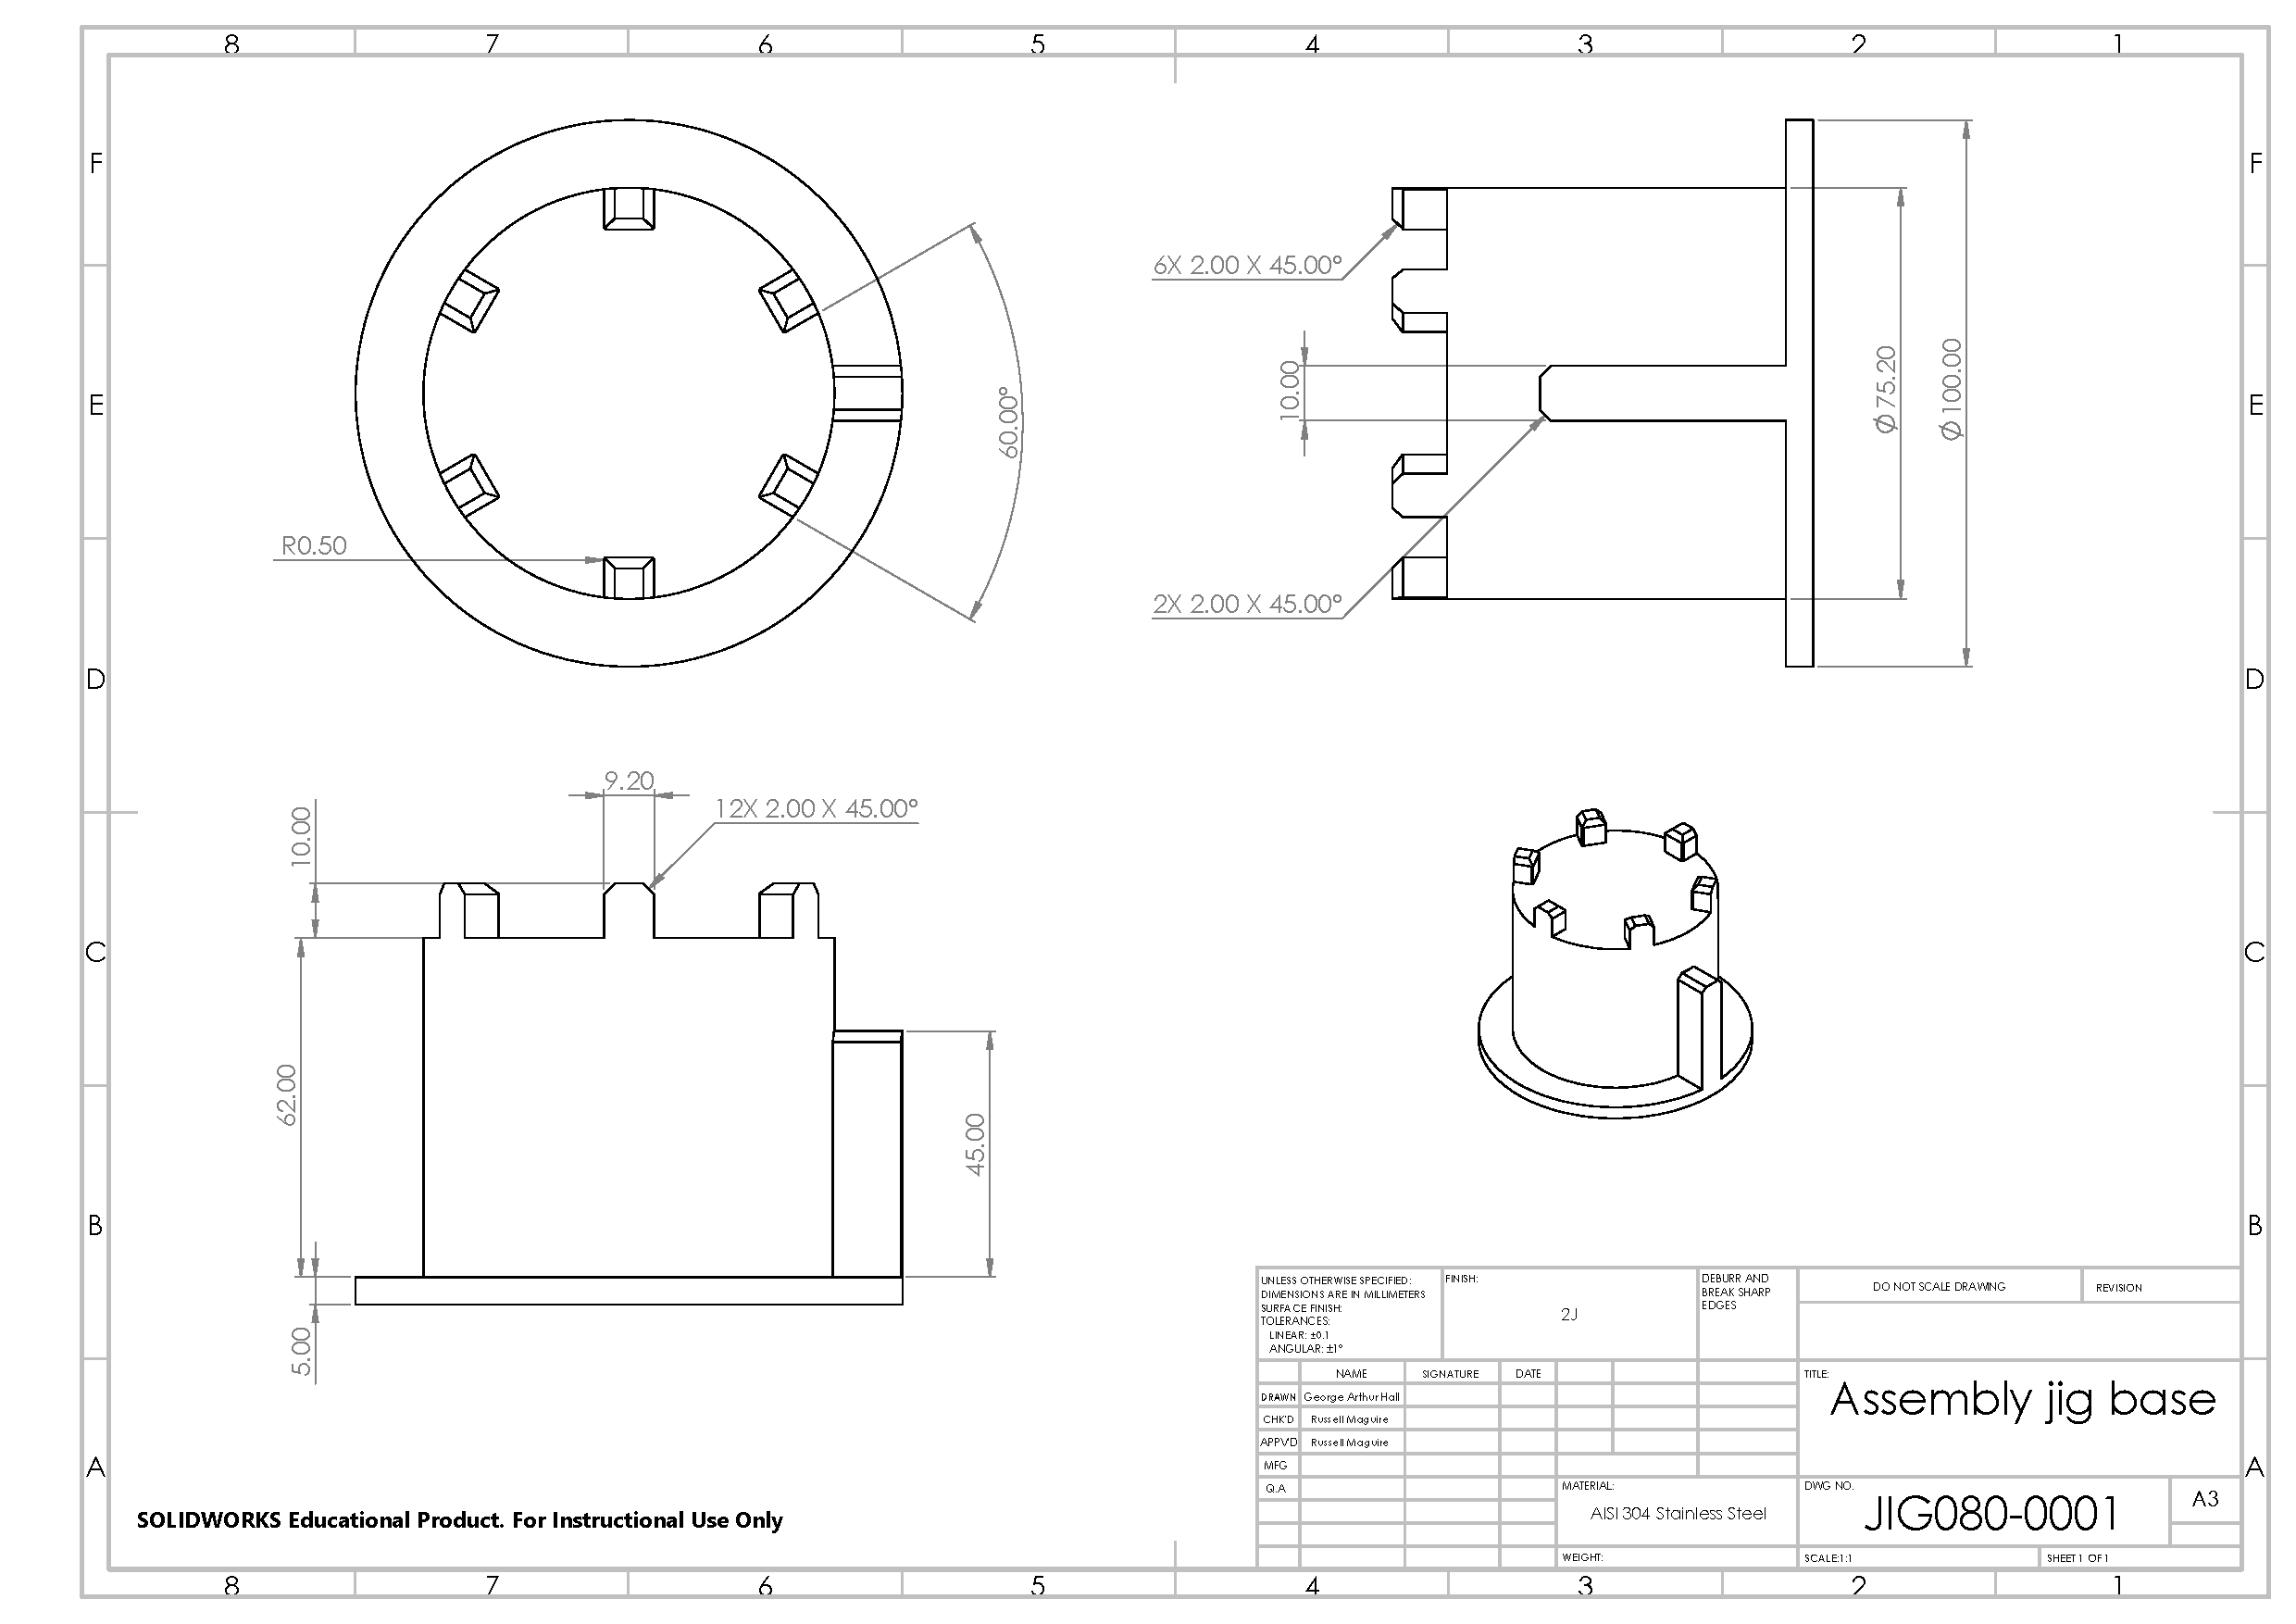
\includepdf[pages=-,fitpaper=true]{Images/jig/JIG080-0001.PDF}
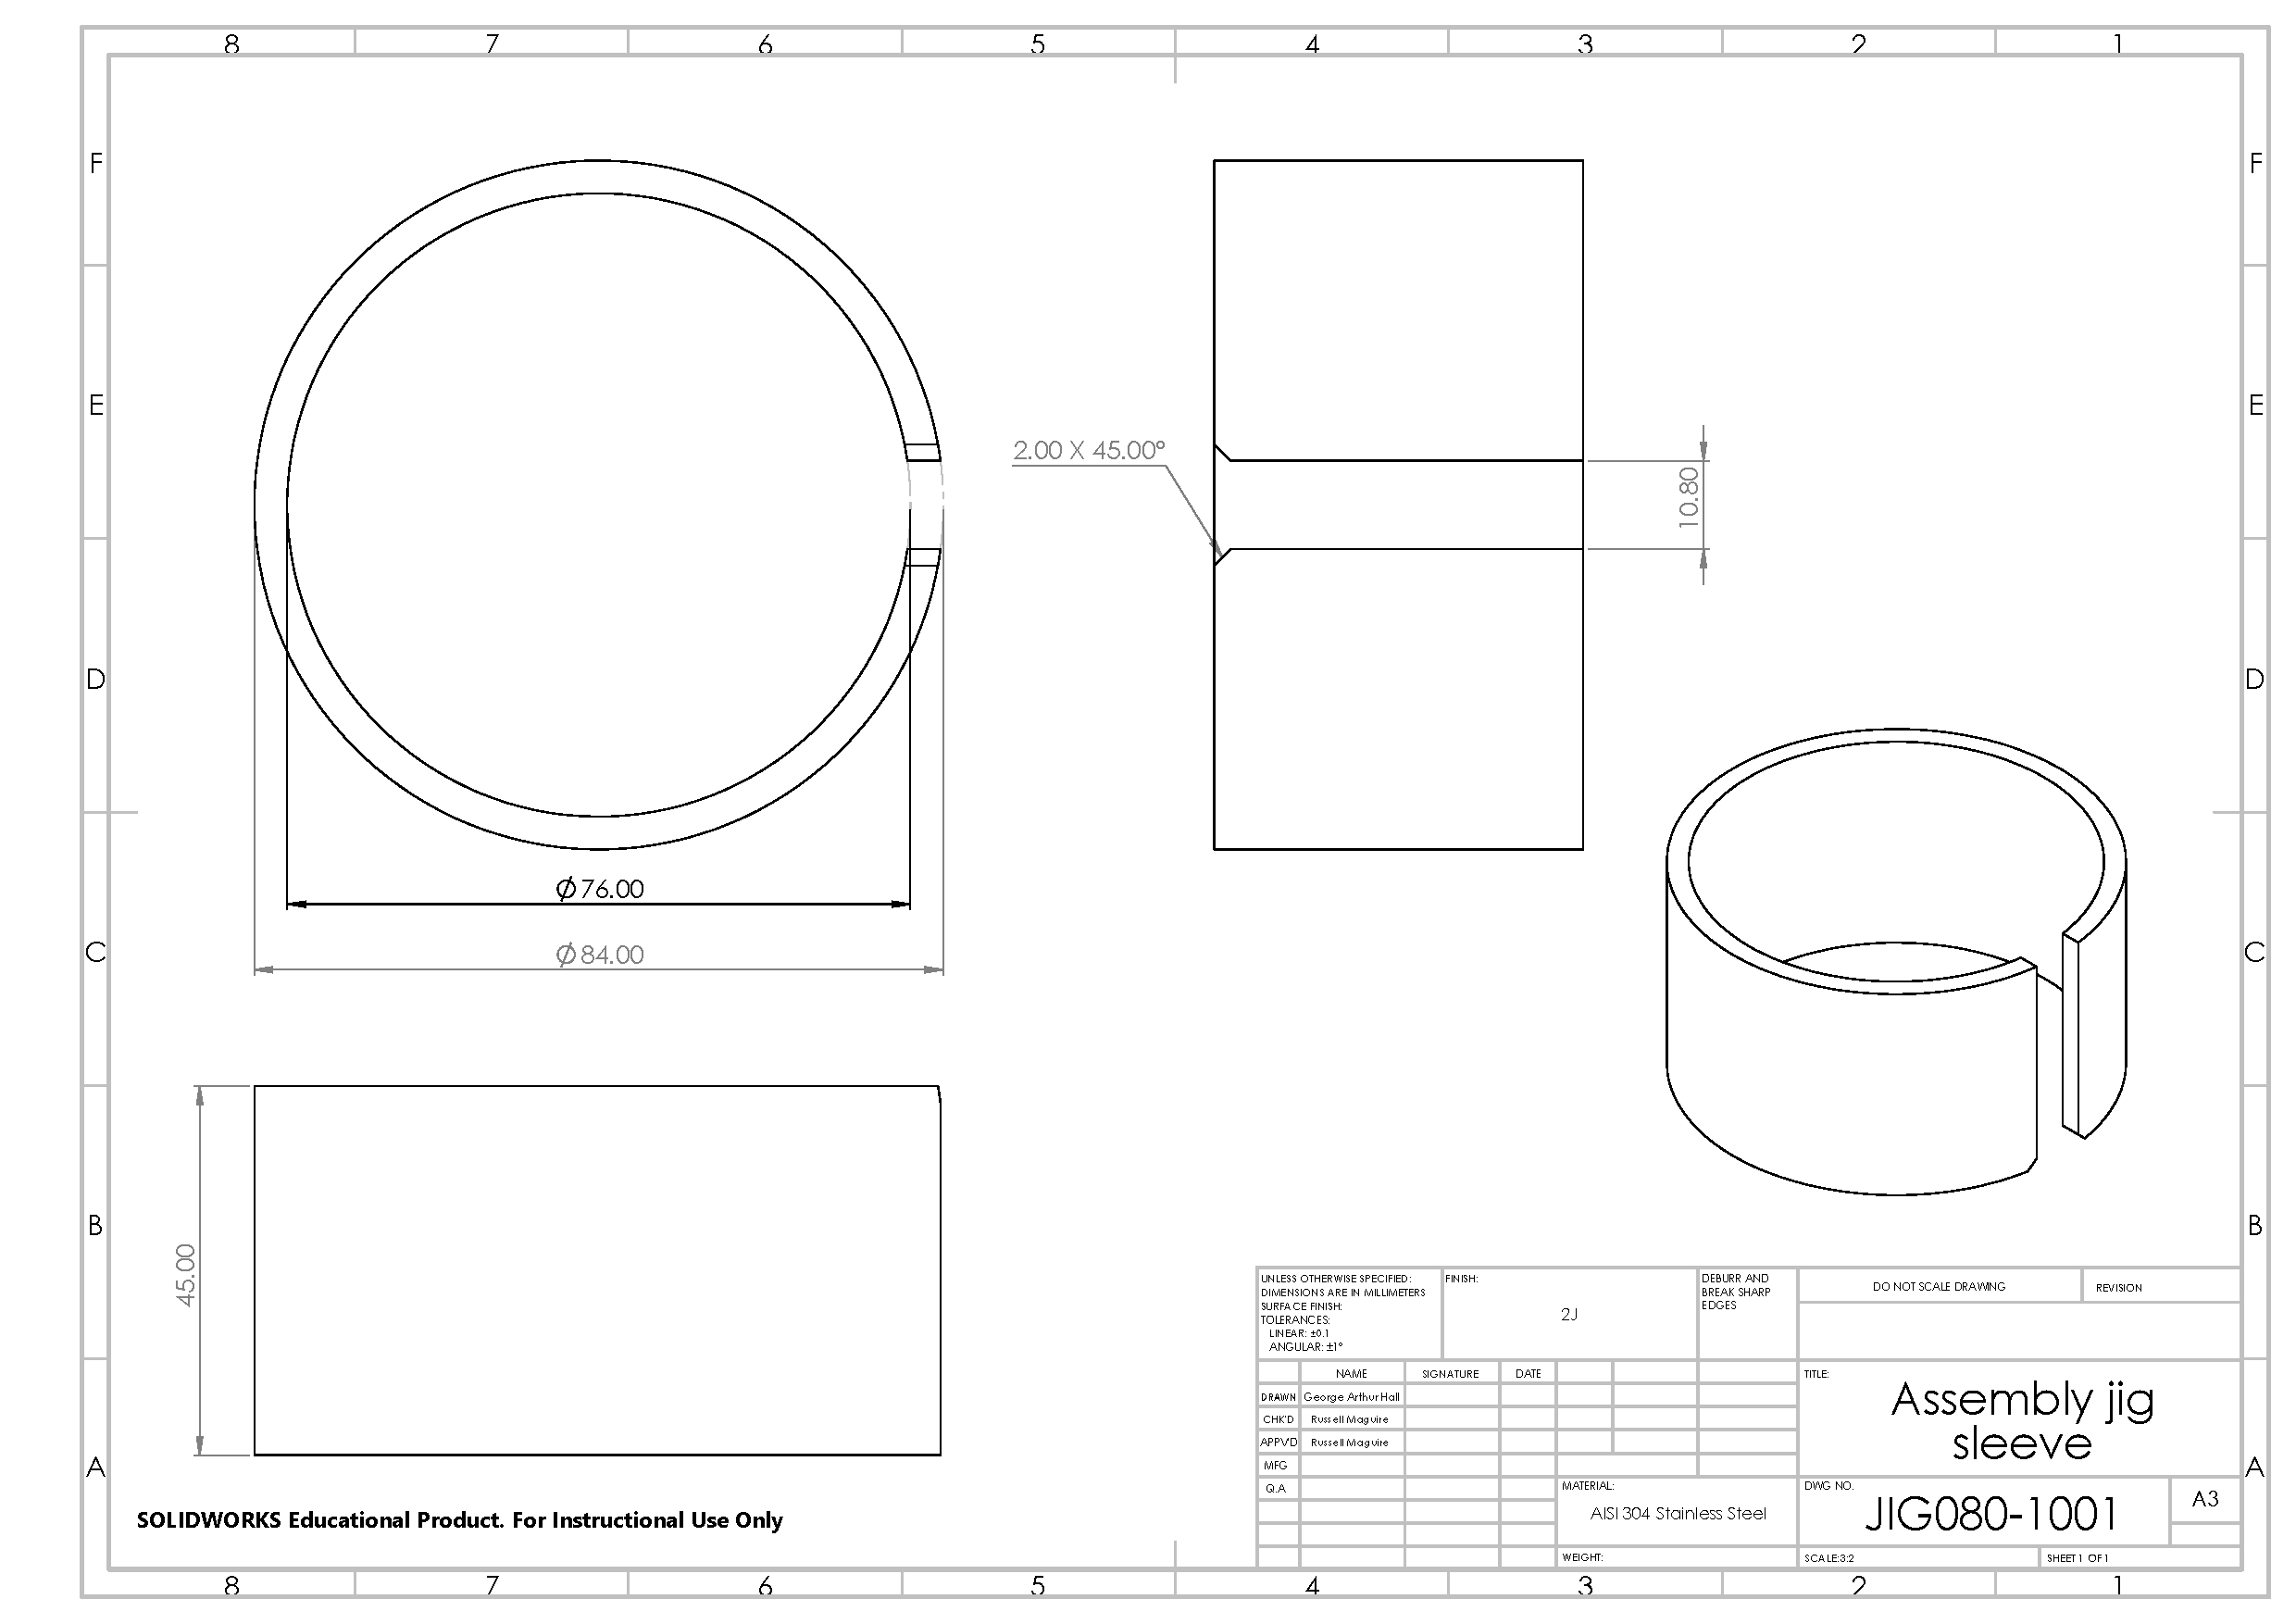
\includepdf[pages=-,fitpaper=true]{Images/jig/JIG080-1001.PDF}

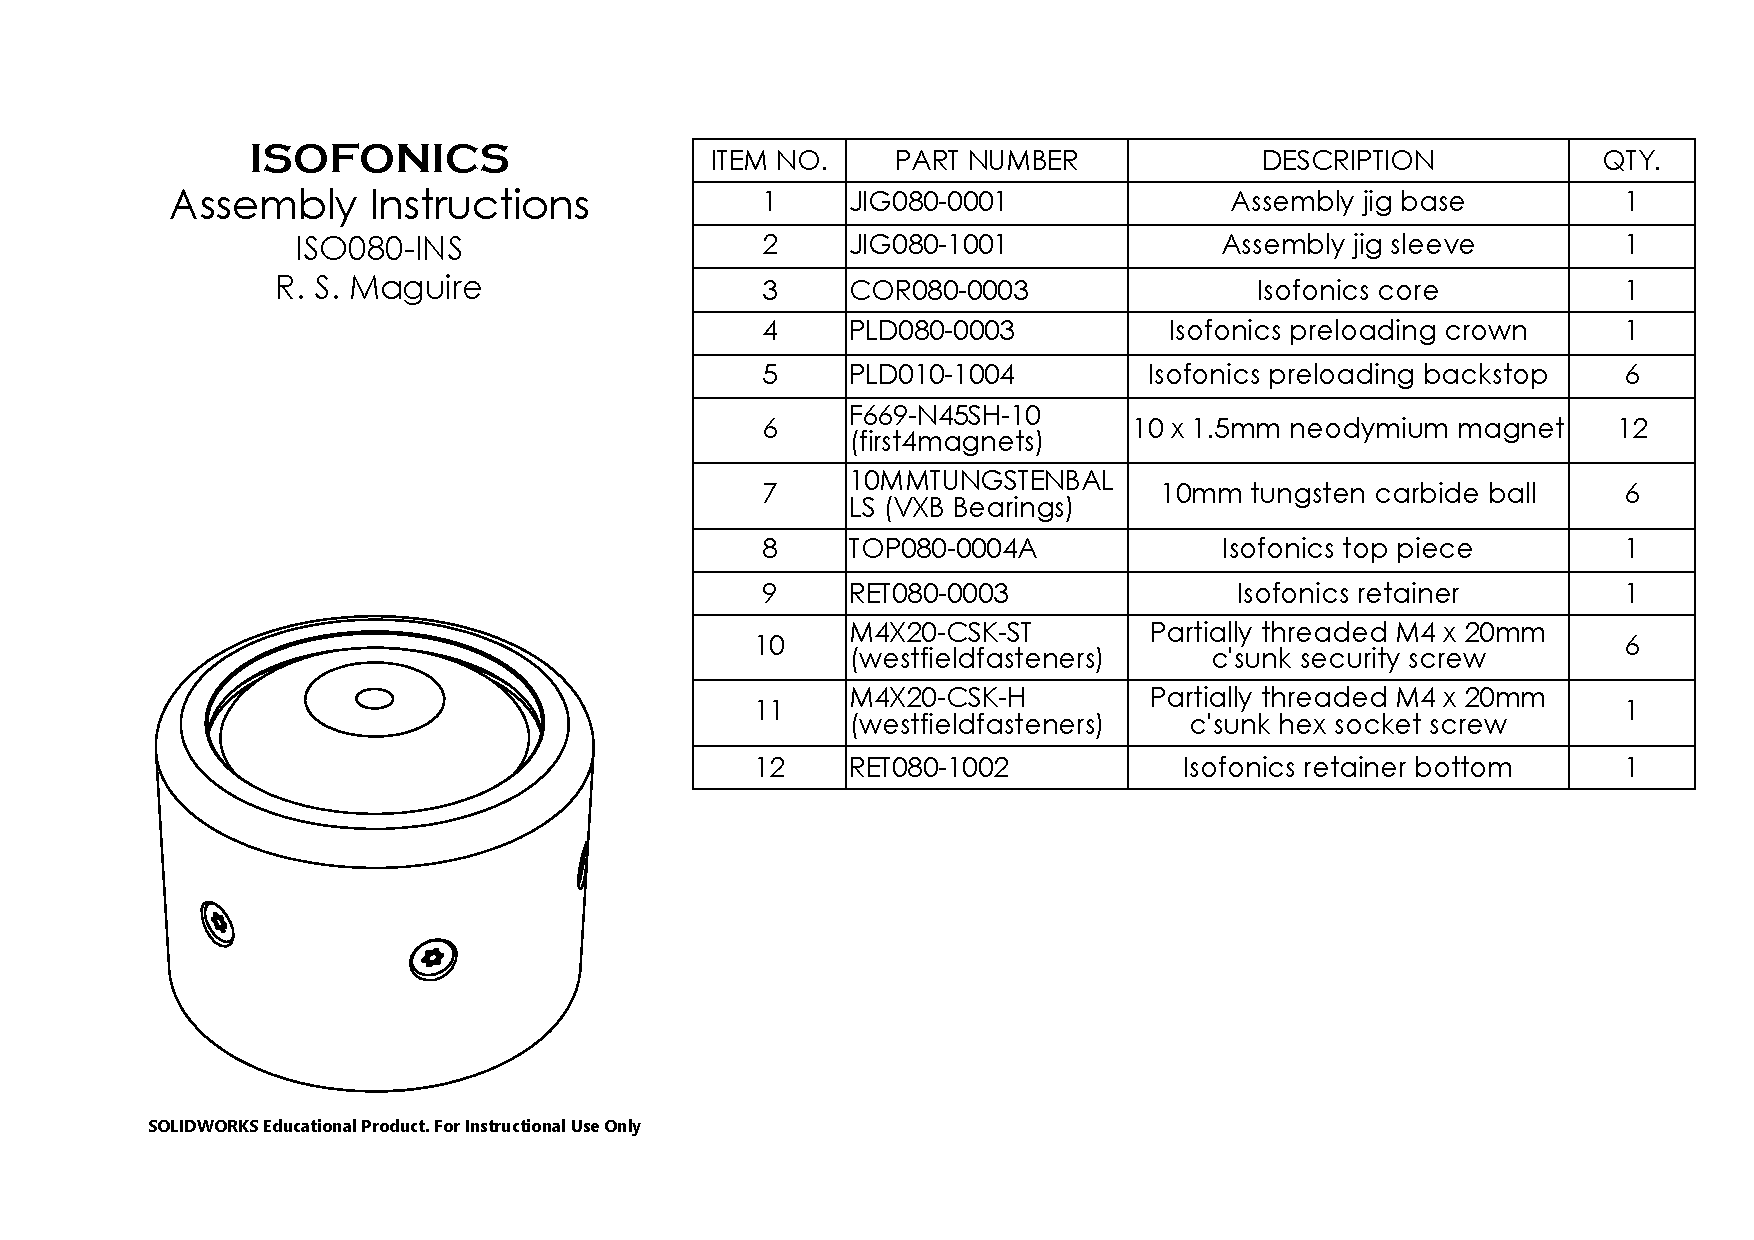
\includepdf[pages=-,fitpaper=true]{Images/jig/ISO080-INS.PDF}



\end{document}
